%To correctly compile this document with its table of contents, glossaries, references, and citations within the glossary when using TexMaker, compile using the following proceedure:

%1) PDFLaTeX
%2) BibTeX
%3) makeglossaries (user command)
%4) PDFLaTeX
%5) PDFLaTeX

%This solution was from http://tex.stackexchange.com/questions/6845/compile-latex-with-bibtex-and-glossaries

% ------------------------------------------------------------------------
% A Latex "template" for CMP MSc Dissertation
% Produced by Dr. Wenjia Wang through modification of 
% Stanford University PhD thesis style file.  
% 
% Brief Instructions
%#### 
% 1. Write your abstract in a separate tex file and name it as ABS.tex
% 2. Write your acknowledgement in a separate tex file and name it as ACK.tex  
%   Note :  Both ABS and ACK files are already included in the style file. 
% 3. wirte each chapter in a separate tex file and name e.g. Ch1, Ch2, etc. 
% and then use "include" to inlcude them as shown in this example.

% Disclaimer: This template is provided as it is 
% You may use it as you wish, 
% but Dr. Wang won't be resposible for resolving any problems it has or causes.
%
% 
% ------------------------------------------------------------------------

\documentclass[12pt]{report}
\usepackage[centertags]{amsmath}
\usepackage{amsfonts}
\usepackage{amssymb}
\usepackage{amsthm}
\usepackage{newlfont}
\usepackage{graphicx}
\usepackage{color}
\usepackage{apalike} % by wjw
\usepackage{pdfsync} %PDF Forward Search
\usepackage[toc]{glossaries} 
\usepackage{CMPDissertation} %CMP Dissertation Style
\usepackage{amsmath}
\usepackage{amsfonts}
\usepackage{amssymb}
\usepackage{color}
\usepackage{url}
\usepackage{pgf}
\usepackage{float}
\usepackage{tikz}
\pagenumbering{arabic}
\usepackage[justification=centering]{caption}
\usepackage{xtocinc} %Include Table of Contents as the first entry in TOC
%                     Faculty of Grad Studies insists on this!?
%\usepackage[active]{srcltx}  %SRC Specials for DVI search
% Fuzz -------------------------------------------------------------------
\hfuzz2pt % Don't bother to report over-full boxes if over-edge is < 2pt
% Line spacing -----------------------------------------------------------
\newlength{\defbaselineskip}
\setlength{\defbaselineskip}{\baselineskip}
\newcommand{\setlinespacing}[1]%
           {\setlength{\baselineskip}{#1 \defbaselineskip}}
\newcommand{\doublespacing}{\setlength{\baselineskip}%
                           {2.0 \defbaselineskip}}
\newcommand{\singlespacing}{\setlength{\baselineskip}{\defbaselineskip}}
\makeglossaries
% MATH -------------------------------------------------------------------
\newcommand{\A}{{\cal A}}
\newcommand{\h}{{\cal H}}
\newcommand{\s}{{\cal S}}
\newcommand{\W}{{\cal W}}
\newcommand{\BH}{\mathbf B(\cal H)}
\newcommand{\KH}{\cal  K(\cal H)}
\newcommand{\Real}{\mathbb R}
\newcommand{\Complex}{\mathbb C}
\newcommand{\Field}{\mathbb F}
\newcommand{\RPlus}{[0,\infty)}
%
\newcommand{\norm}[1]{\left\Vert#1\right\Vert}
\newcommand{\essnorm}[1]{\norm{#1}_{\text{\rm\normalshape ess}}}
\newcommand{\abs}[1]{\left\vert#1\right\vert}
\newcommand{\set}[1]{\left\{#1\right\}}
\newcommand{\seq}[1]{\left<#1\right>}
\newcommand{\eps}{\varepsilon}
\newcommand{\To}{\longrightarrow}
\newcommand{\RE}{\operatorname{Re}}
\newcommand{\IM}{\operatorname{Im}}
\newcommand{\Poly}{{\cal{P}}(E)}
\newcommand{\EssD}{{\cal{D}}}
% THEOREMS ---------------------------------------------------------------
\theoremstyle{plain}
\newtheorem{thm}{Theorem}[section]
\newtheorem{cor}[thm]{Corollary}
\newtheorem{lem}[thm]{Lemma}
\newtheorem{prop}[thm]{Proposition}
%
\theoremstyle{definition}
\newtheorem{defn}{Definition}[section]
%
\theoremstyle{remark}
\newtheorem{rem}{Remark}[section]
%
\numberwithin{equation}{section}
\renewcommand{\theequation}{\thesection.\arabic{equation}}
%%% ----------------------------------------------------------------------
\setlength{\tclineskip}{1.05\baselineskip}
%%% ----------------------------------------------------------------------
%\nobib
%\draft
%\nofront

%\permissionfalse

\dedicate{}

%\nolistoftables
%\nolistoffigures

\msc

%\phd
\university{The University of East Anglia}
\school{Computing Sciences}

%#### CHOOSE OR INSERT YOUR MSC COURSE TITLE BELOW #####
% by commentting in your course from the liste befow.

\course{Computing Science}

\copyrightyear{2017} %Check that this is correct
\submitdate{August 2015}
%\convocation{October}{2012}

% ------------------------------------------------------------------------
% #### Insert the title of your dissertation below.#####
\title{Data Centre Modelling}

% #### Insert your full name below.#####
\author{Daniel Pawsey}

%#### insert your supervisor's name below #####
\supervisor{ Dr. D. Smith}

%#### insert the name of your markers if you know them #####
\firstmarker{Marker 1: Dr. xxxxxx}
\secondmarker{Marker 2: Dr. xxxxxx}
\examiner{Checker/Moderator}
\organiser{Dr. Wenjia Wang}

% ------------------------------------------------------------------------
\begin{document}
{
\typeout{:?000000000} % Don't bother with over/under-full boxes
\beforepreface
\typeout{:?111111111} % Process All Errors from Here on
}

\afterpreface
\def\baselinestretch{1}
\setlinespacing{1.66}

% ------------------------------------------------------------------------
% ##### Include each chapter in order below #####
% ------------------------------------------------------------------------
% -*-TeX-*- -*-Hard-*- Smart Wrapping
% ------------------------------------------------------------------------
\def\baselinestretch{1}

\chapter{Background and Study Plan}
\label{chapter:Intro}

\def\baselinestretch{1.66}


%%% ----------------------------------------------------------------------

\textcolor{red}{[GIVE A CHAPTER DESCRIPTION]}

%%% ----------------------------------------------------------------------
\goodbreak
\newglossaryentry{data centre}
{
  name=Data Centre,
  description=
  {
     A data centre is defined as being any space dedicated to the purpose of housing an
     organisation's ICT infrastructure \cite{InteraxionWhatIsADataCentre}. In the strictest terms, this
     definition can refer to any collection of equipment serving this purpose for an organisation, modern
     \emph{data centres} tend to include vast arrays of equipment to support the operation of their ICT
     equipment, such as strict environmental and airflow control, uninterruptable power supplies, and
     fire suppression equipment 
     \cite{PaloAltoWhatIsADataCentre}\cite{DataCenterDefinitionGartnerITGlossary}
  }
}
     
\section{Background}
\label{sec:Background}
With the rise of cloud computing services, streaming video services such as Youtube, audio streaming services such as Spotify, and a host of other services, the world has seen a dramatic increase reliance on \gls{data centre}s. Naturally, \gls{data centre} traffic has increased with these developments, with Cisco Systems reporting a 21\% increase in global \gls{data centre} IP traffic between 2012 and 2013 (at 3.3 Zettabytes per year for 2013), with a projected rise of an additional 21\% between 2013 and 2014 \cite{CiscoGlobalCloudIndex:ForecastAndMethodology}.


\begin{figure}[H]
\centering
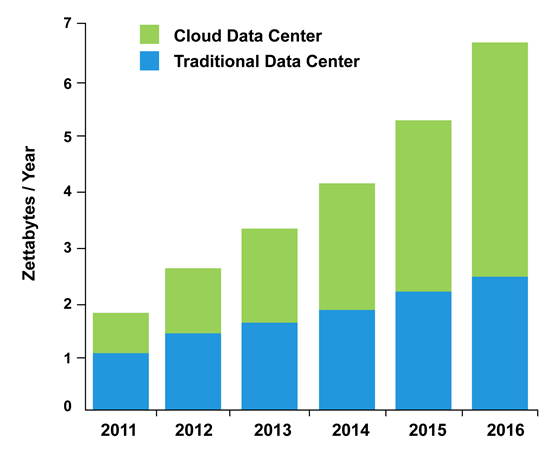
\includegraphics[width=5in]{Resources//1.png}
\caption{Image source: http://thirdmillenniumtimes.com/ \cite{ThirdMilleniumTimesInternetIsStillGrowingFast}, Web page representation of image acknowledges data source as Cisco Global Cloud Index: Forecast and Methodology, 2012–2017 \cite{CiscoGlobalCloudIndex:ForecastAndMethodology}.}
\label{fig:ThirdMilleniumTimesBarGraph}
\end{figure}

Naturally, this increase has lead \gls{data centre}s to become major users of electricity, with ever increasing demand for better processors and more storage in the systems located therein. Koomey shows that of all electricity used globally in 2005, 1\% of it was used in the operation of \gls{data centre}s, which is an increase from the 2000 figure of 0.5\% \cite{KoomeyGrowthInDataCenterElectricityUse}.

This presents a conundrum: cloud-computing and other \gls{data centre} dependant technologies are becoming ever more popular, which is driving \gls{data centre}s to become less sustainable in terms of general energy consumption. \textcolor{red}{Therefore, it is necessary to take steps towards bringing \gls{data centre}s in line with energy efficiency goals.[UPDATE THIS WITH TEXT FROM THE PRESENTATION}

\subsection{Goals of this Project}
\label{sec:Background:GoalsOfThisProject}
This project aims to produce a game in which the user must outfit a data centre. This will follow the format of being a strategy game, which will consider the following principles in its design:

\begin{itemize}

\item In order to present this game to as wide an audience as possible it will be developed as an internet-browser based game \textcolor{red}{, and, upon completion of this aspect of it, may be ported to mobile gaming platforms such as Android and ios.}

\item This game will require users to take account of energy-efficiency, cost-effectiveness and operational efficiency of their data centre while they design it.

\item In order to fulfil these goals, players of the game will require users to select components for their \gls{data centre} as they set it up, each of which will have an impact on an overall aggregate score for the \gls{data centre}, which will be derived using the three criteria mentioned above.

\end{itemize}

\subsubsection{Justification}
\label{sec:ProjectGoal:Justification}
The justifications for this project are twofold:

\begin{enumerate}
\item To bring awareness of cloud-computing environmental concerns to Internet users, doing so by providing the information in an accessible format.

\item To provide a means of demonstrating what is required to design a data centre in a format accessible to general users.
\end{enumerate}

\subsection{Study Plan}
\label{sec:Background:StudyPlan}
This study will consist of the following elements in the following sequence:

\begin{enumerate}
\item A literature review of real world concepts and technologies relevant to this project. These will include the following:
\begin{itemize}
\item Studies into the environmental effect of \gls{data centre}s, seeking to ascertain the chief concerns in this area so that appropriate ways of modelling them in the game can be devised.

\item Studies into the energy efficiency and cost effectiveness of devices and elements of \gls{data centre}s, such as Central Processing Units (CPUs), cooling systems, storage systems, memory systems etc.

\item Studies into the application of Artificial-Intelligence in strategy games such as Sim-City, Civilization and The Sims. \textcolor{red}{CITE THESE GAME NAMES.}

\item Studies of browser-games developed using JavaScript.
\end{itemize}

\item With the information gathered from section \ref{sec:ACriticalReviewOfReleventScientificAndEngineeringLiturature}, a three-part game platform will be developed. These parts are as follows:
\begin{enumerate}
\item A database of elements to be used in game, representing real world components and elements used within the \gls{data centre}. An example would be a \textcolor{red}{CPU type[BAD EXAMPLE, GO WITH SERVER AND UP]}, which would itself have attributes such as optimal operating temperature in degrees Celsius, speed in gigahertz, cost in US dollars and energy consumption in kilowatt-hours. Another example would be a particular cooling system, which would have attributes such as temperature reduction in degrees Celsius and energy consumption in kilowatt-hours.

\item A database of logic and rules to be checked in game-play. Such rules could include the following:
\begin{itemize}
\item \textcolor{red}{If a CPU has a set temperature at which it overheats, and lacks an adequate cooling system to prevent it exceeding this temperature, a rule should be included to say that  the CPU will malfunction. Other rules would link into this, for example, the loss of this CPU could lead the overall operating speed of the data-center to fall, which could lead the reputation of the data-center with customers to fall also.[BAD EXAMPLE: GO WITH SERVER AND UP]}

\item Operating more processors at night time when it is cooler could lead to lower costs due to lower temperature, but may lead to a drop in the \gls{data centre}'s reputation with customers due to inconsistent speeds.
\end{itemize}

\item A basic test program, allowing the user to input commands such as to use a certain type of CPU, seeing how the logic-engine part of the program
responds under different conditions.
\end{enumerate}

\textcolor{red}{Specifically, the test program, and later the game platform itself will be written in JavaScript, allowing dynamic user interaction. This will be embedded in a page utilising CSS and HTML5 coding.}

\item 
This test-program will be tested under differing conditions. This will serve as a white-box test of the component database and the logic engine elements of the application.

\item An interface between the database and logic-engine components of the application will be developed, along with a Graphical User Interface (GUI).

\item The program will undergo a final stage of testing.
\end{enumerate}
% ------------------------------------------------------------------------
% -*-TeX-*- -*-Hard-*- Smart Wrapping
% ------------------------------------------------------------------------
\def\baselinestretch{1}

\chapter{A Critical Review of Relevant Scientific and Engineering Literature}
\label{chapter:LitReview}

\def\baselinestretch{1.66}


%%% ----------------------------------------------------------------------

This chapter details research into various areas relevant to the project, forming a factual basis for assumptions made later in the system development (chapter \ref{chapter:Development}).

%%% ----------------------------------------------------------------------
\goodbreak

\subsection{Studies into the Environmental Effects And Energy \newline Efficiency of Data-Centres}
\label{sec:ACriticalReviewOfReleventScientificAndEngineeringLiturature:StudiesIntoTheEnvironmentalEffectsAndEnergyEfficiencyOfDataCenters}

In the study \textbf{GreenDCN: a General Framework for Achieving Energy Efficiency in Data Centre Networks}, \emph{Lin Wang et al.} demonstrate that, in addition to available devices, traffic routing techniques can be considered for the purposes of ensuring more energy-efficient operation of data centres \cite{GreenDCN}. Specifically, either predictive or, perhaps more sensibly, an EER algorithm designed to direct traffic to lesser taxed areas of the network. Furthermore, the paper illustrates that the switches themselves consume power, but switching them off when appropriate saves power, and this is a dynamic that can be modelled in the game application.

Lin Wang et al. \cite{GreenDCN} argue that ordinary methods of data centre
traffic engineering and prediction can be inaccurate, and instead propose an Energy-
Efficient Routing (EER) Algorithm, which uses \cite{multipath routing protocol}, MPTCP
in order to distribute network traffic across pathways which are less taxed at a given time, with an emphasis on avoiding overtaxed areas, weighting assignment against those pathways.

In the same study \cite{GreenDCN}, there is also a section titled \emph{Modelling The Energy-Saving Problem}, which details the difference between energy saving techniques that can be used for a single network data centre, and those with more than one network. The section also discusses the physical means in which power is saved: The network is described as a series of switches, v between servers, and to keep one open requires power proportional to the transmission speed of the switch. Within the game, both the EER and the switching mechanism can be represented as in game rules.

The experimental results of Lin Wang et al’s study are thorough in their scope, however, the parameters are limited: A single laptop is used on a single network with a pre-defined power supply is used to test the experimenter's algorithm against others. It would be appropriate to repeat the experiment using different hardware so as to generalise the findings to other networks and different situations \cite{GreenDCN}.
\\

The study \textbf{Report to congress on server and data center energy efficiency public law 109-431} \cite{USCongressDataCenterEfficiencyReport} makes an interesting point about the improvement in microprocessor technology between 1986 and 2002, simultaneously increasing in energy efficiency and increasing the demand for them in data centre contexts, which has actually lead to an increase in use of electricity by data centres in the US  \cite[3.1 Expected Energy Savings from Current Energy Efficiency Trends]{USCongressDataCenterEfficiencyReport}. Therefore, in modelling CPU choice for devices in game, it is important to observe this trend and note that with more energy efficient devices comes the temptation to use more of them to increase performance.

This section of the paper goes on to discuss the use of multi-core processors, containing two or more cores running at lower frequencies than equivalent single-core processors. The paper claims that the shift towards multi-core processors in data centres will lead to an increase in overall data centre energy efficiency as multi-core processors are more efficient than equivalent single-core processors. There are two issues with this claim: The paper simply claims that multi-core processors are ``more energy-efficient", without quantifying whether this is because they use less electricity in kilowatt-hours, whether they waste less energy by generating heat, or due to some other factor. Furthermore, this claim seems to contradict the paper's claim that the shift in energy-efficiency of modern microprocessors has led to greater demand for the devices, driving down the overall energy efficiency of data centres in the US \cite[3.1 Expected Energy Savings from Current Energy Efficiency Trends]{USCongressDataCenterEfficiencyReport}.

This section of the paper goes on to make further claims that developments in memory and storage devices may lead to overall greater energy efficiency in data centres in the US.

Furthermore, the study makes some optimistic claims about technological developments and the energy savings this could lead to \cite[3.1 Expected Energy Savings from Current Energy Efficiency Trends]{USCongressDataCenterEfficiencyReport}, however, it is important to note that this is research commissioned and funded by a national government to advise it on how it should spend resources and make policies relating to the problem of energy efficiency in data-centers, so could be considered to be biased towards a particular course of action.

The EPA's claims \cite[3.1 Expected Energy Savings from Current Energy Efficiency Trends]{USCongressDataCenterEfficiencyReport} about multi-core processors are interesting and could be modelled in the game, however, it is important to note the contradictions which that section of the paper makes, which does imply that further research into the energy efficiency of multi-core processors when compared to single-core processors is required.
\\

In \textbf{Improving Data Center Energy Efficiency Through Environmental Optimization} \textcolor{red}{[NOTE: CHECK THAT THIS IS THE NAME OF THE STUDY]}, \emph{Seeber and Seeber} \cite{SeeberAndSeeberImprovingDataCenterEnergyEfficiencyThroughEnvironmentalOptimization} performed a study into the influence of various environmental factors on the operational efficiency of data centre computing equipment. The study is an industrial white paper published by \emph{Mid Atlantic Infrared Services, Inc.}, which are a company who sell equipment and services to control the environment of data centres and such IT systems housings \cite{MidAtlanticInfraredWebsite}. As such, the study may have the agenda of selling these products, influencing what is claimed.

\newglossaryentry{CRAC}
{
  name=CRAC,
  description={Acronym of \emph{Computer Room Air Conditioner}, an air conditioning system which takes in air, passes it over a refrigerant-filled coil, and expels the cooled air back out into the \gls{data centre}. It works in a very similar manner to a household or office air conditioning unit \cite[CRAC]{DataCenterHuddleCRACVsCRAHDefinition}. Many   configurations for \emph{CRAC} systems have been used, including systems that intake warm air through ceiling vents where it is refrigerated, before using fans to blow it back into the room through floor vents \cite{CRACDefinition-SearchDataCenter}}
}

\newglossaryentry{CRAH}
{
  name=CRAH,
  description={Acronym of \emph{Computer Room Air Handler}, these differ from CRAC units by using fans and water cooling systems, rather than air refrigerators \cite{CRAHDefinition-SearchDataCenter}}
}

The study describes a process called \emph{Environmental Optimisation}, which it describes as being the regulation of humidity, airflow and established set points for air temperature within a \gls{data centre}. The article claims that the right combinations of these factors can lead to substantial energy savings \cite[abstract]{ SeeberAndSeeberImprovingDataCenterEnergyEfficiencyThroughEnvironmentalOptimization}.

The paper claims that of critical importance is the interdependence of the criteria of air flow, temperature and humidity. Furthermore, it describes the following potential risks of a non \emph{environmentally optimised} data centre:

\begin{itemize}

\item Increasing the flow of air over a server rack that is too hot or too humid could damage the equipment.

\item Increasing humidity without concern for temperature may lead to inefficient operation or damage to equipment due to condensation within equipment.

\item A humidity that is too low may lead to equipment damage through electrostatic discharges.

\end{itemize}

\newglossaryentry{recirculation}
{
  name=Recirculation,
  description={in the context of data centre \emph{environmental optimisation} as discussed in section \ref{ sec:ACriticalReviewOfReleventScientificAndEngineeringLiturature:StudiesIntoTheEnvironmentalEffectsAndEnergyEfficiencyOfDataCenters:WSeeberAndSSeeberImprovingDataCenterEfficiencyThroughEnvironmentalOptimization}, \emph{recirculation} refers to the undesired effect of warm air failing to pass into a warm air inlet, instead circulating back into the room it has already been used to cool. This somewhat negates any prior cooling effect the formerly cool air warms the same equipment it has already cooled. Not only can this damage equipment, it is also an inefficient use of energy, as its desired cooling effect is not achieved \cite{SeeberAndSeeberImprovingDataCenterEnergyEfficiencyThroughEnvironmentalOptimization}\cite{BanuelosManagingDataCentreHeatIssues}}
}

\cite{ SeeberAndSeeberImprovingDataCenterEnergyEfficiencyThroughEnvironmentalOptimization} claims that by using perforated tiles over \gls{CRAC} and \gls{CRAH} air inlets, the air temperature set points for the overall \emph{environmental optimisation} of the data centre can be raised, increasing the overall \textcolor{red}{energy efficiency} of the data centre by reducing the load on the \gls{CRAC} or \gls{CRAH} \textcolor{red}{[YOU NEED TO INCLUDE A DEFINITION OF ENERGY EFFICIENCY IN YOUR BACKGROUND, AND A STANDARD AGAINST WHICH TO MEASURE DATA CENTRES AGAINST IT]} \cite[abstract]{ SeeberAndSeeberImprovingDataCenterEnergyEfficiencyThroughEnvironmentalOptimization}. \textcolor{red}{[USE STUDY RESULTS TO CHECK AND CRITICISE THIS CLAIM]}

The paper recommends a list of constraints to consider when implementing either a \gls{CRAC} or a \gls{CRAH} system in a \gls{data centre}. These include  ensuring that equipment remains below its manufacturer's recommended maximum operating temperature \textcolor{red}{(implying that the whole \gls{data centre} (or at least each individual zone within it) should not be allowed to increase in temperature above the maximum temperature of its constituent component with the lowest manufacturer recommended maximum operating temperature)}, ensuring proper airflow is maintained, and that enough warm-air inlets are available in the appropriate locations.

The aforementioned criteria mean that an important concern is that greatest energy efficiency in any \gls{data centre} cooling system is achieved when the correct balance of air inlets (through perforated tiles) proving an optimum airflow is achieved \cite[Optimizing Air Temperature Set Points and Air Flows Can Shrink PUE Numbers]{SeeberAndSeeberImprovingDataCenterEnergyEfficiencyThroughEnvironmentalOptimization}

Infra-red mosaic data provided in \cite[Optimizing Air Temperature Set Points and Air Flows Can Shrink PUE Numbers]{SeeberAndSeeberImprovingDataCenterEnergyEfficiencyThroughEnvironmentalOptimization} scientifically support the paper's claim that hot air \gls{recirculation} leads to server hot spots, which represents inefficient cooling, and a potential risk to equipment within the \gls{data centre}. A strength of the development of these images is that they do show the results of this effect on 440 servers within racks in a typical \gls{data centre} layout. \textcolor{blue}{[}\textcolor{red}{THE FOLLOWING MIGHT BE GOOD, BUT REVIEW, MAYBE ITS IRRELEVANT:}\textcolor{blue}{The study says that the authors have developed techniques to create the infra-red mosaics displayed (figure \ref{fig:SeeberAndSeeberIRMosaics}), displaying an entire \gls{data centre} floor. It is scientifically useful that their study used a single data centre however, there appears to have been no repetition of the study to produce similar Infra-Red mosaics for other data centres, thus, it is not possible to rule out anomalous effects outside of the scope of the study of the data centre studied leading to false results. Furthermore, the paper does not explain how the technique for building the Infra-Red mosaic images work, meaning that their validity is questionable, particularly as t}his study is a white paper: It must be considered that this study and these techniques could be biased to support an agenda of the author.

\begin{figure}[H]
\centering
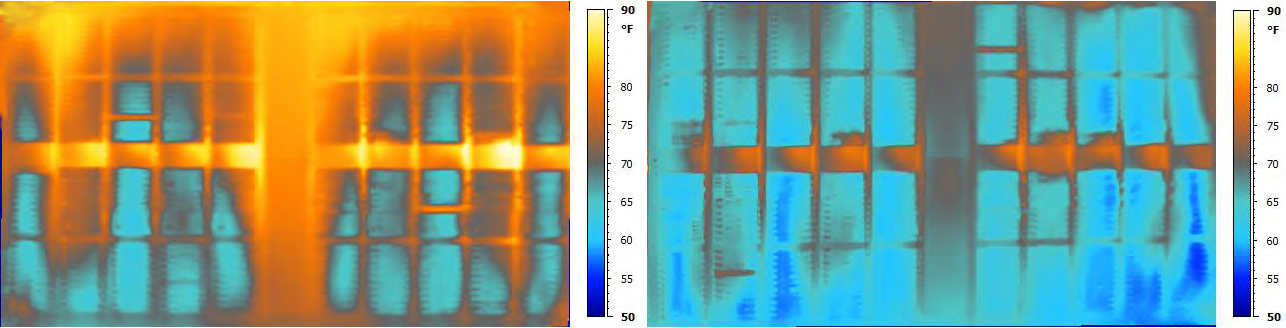
\includegraphics[width=5in]{Resources//S Seeber and W Seeber- IRMosaicImages.png}
\caption{The Infra-Red mosaic images created for the study. The left hand image shows the result of over-cooling, and the right hand image shows the result of over cooling: The study claims that both of these effects are the result of poor air circulation in different contexts \cite[Optimizing Air Temperature Set Points and Air Flows Can Shrink PUE Numbers]{SeeberAndSeeberImprovingDataCenterEnergyEfficiencyThroughEnvironmentalOptimization}.}
\label{fig:SeeberAndSeeberIRMosaics}
\end{figure}

This study also includes airflow and air temperature data visualised using a technique called \emph{Data Center Airflow Measurement and Mapping (DAMM)}, a patented technique developed by the paper's institution \cite{SeeberAndSeeberImprovingDataCenterEnergyEfficiencyThroughEnvironmentalOptimization}, which uses data gathered about airflow and temperature with in the \gls{data centre} for these visualisations, which provides an indication of the effectiveness of cooling systems mentioned in the paper \cite[Optimizing Air Temperature Set Points and Air Flows Can Shrink PUE Numbers]{SeeberAndSeeberImprovingDataCenterEnergyEfficiencyThroughEnvironmentalOptimization}.

The DAMM visualisation shown in figure \ref{fig:SeeberAndSeeberDAMM} may be useful as inspiration for the development of an overlay for the program's GUI, showing airflow concerns in the user's \gls{data centre} design, as the visualisation of air flow and temperature as arrows being interpretable to the lay person.


\begin{figure}[H]
\centering
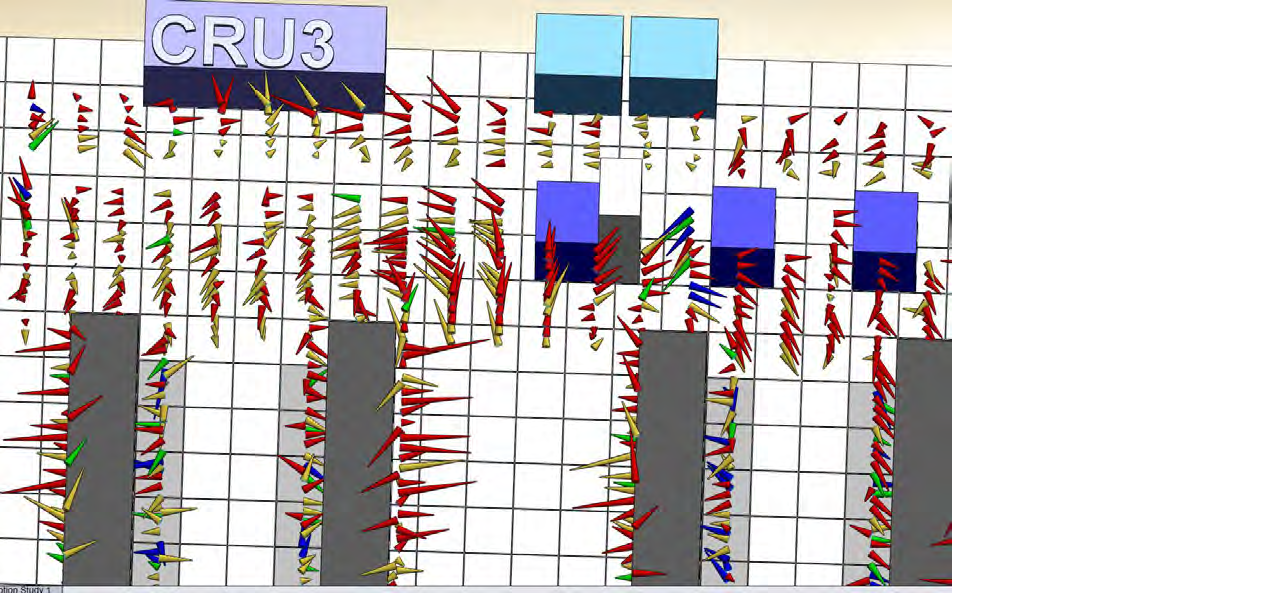
\includegraphics[width=5in]{Resources//SeeberAndSeeberDAMMImage.png}
\caption{
The DAMM visualisation of airflow and temperature within a data centre \cite[Optimizing Air Temperature Set Points and Air Flows Can Shrink PUE Numbers]{SeeberAndSeeberImprovingDataCenterEnergyEfficiencyThroughEnvironmentalOptimization}. Red arrows show temperatures above 80.6$\,^{\circ}F$, while blue arrows indicate that air temperature is below 64.4$\,^{\circ}F$. The direction and length of the arrows represent the direction and velocity respectively of measured air currents. respectively, resumed at the point at which they terminate (their blunt end).}
\label{fig:SeeberAndSeeberDAMM}
\end{figure}

The paper also contains data suggesting that increasing airflow can reduce the incidence of hot spots due to hot air \gls{recirculation} within data centre equipment. A study within the paper shows the propagation of hot spots within equipment included in their study as a temperature of 2$\,^{\circ}F$ was applied, however, the hot spots were abated by increasing airflow by 1000 Cubic Feet per Minute ($CFM$).
The study indicates that this decrease in recirculation becomes less effective at airflows below 5000 $CFM$, which is displayed in a graph (see figure \ref{fig:SeeberAndSeeberAirflowEffectivenessGraph}) \cite[The Numbers: How Much Can You Really Save Through Environmental Optimization?]{SeeberAndSeeberImprovingDataCenterEnergyEfficiencyThroughEnvironmentalOptimization}.

\begin{figure}[H]
\centering
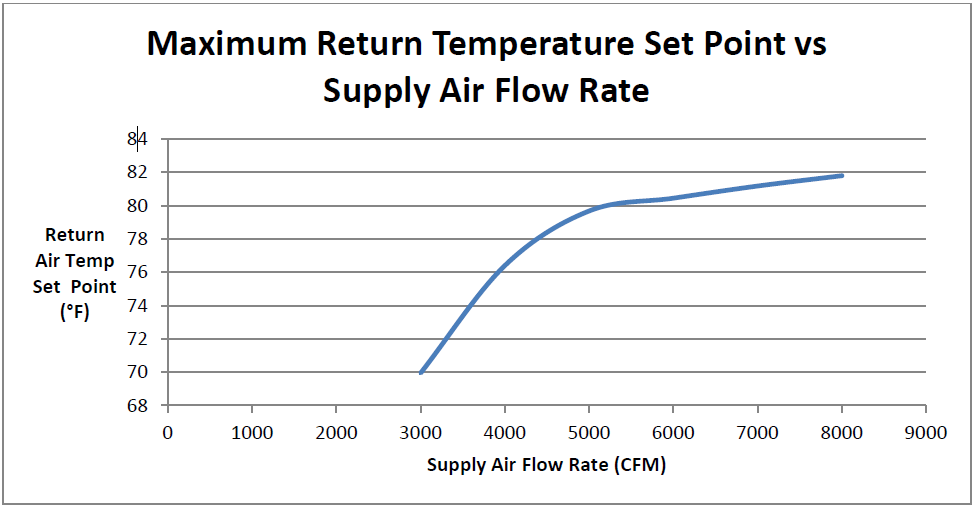
\includegraphics[width=5in]{Resources//SeeberAndSeeberAirflowEffectivenessGraph.png}
\caption{Graph from \emph{Seeber and Seeber's} paper showing the relationship between the supply air flow rate and the return air temperature set point required. The graph shows that for air flow rates above 5000 $CFM$, there is less reduction in return air temperature set point per single $CFM$ of airflow increase, meaning that it is less energy efficient to increase airflow above that threshold because the energy consumed in doing so will increase at the same rate, but the threshold at which the air will need to be cooled will not increase at the same rate as if it were below 5000 $CFM$ \cite[The Numbers: How Much Can You Really Save Through Environmental Optimization?]{SeeberAndSeeberImprovingDataCenterEnergyEfficiencyThroughEnvironmentalOptimization}.}
\label{fig:SeeberAndSeeberAirflowEffectivenessGraph}
\end{figure}

\emph{Seeber and Seeber's} paper also discusses \emph{leekage}, which is defined as airflow that enters a room from any area other than the perforated floor tiles through which air is supposed to flow between the room and the \gls{CRAC} or \gls{CRAH}. This can cause air to flow in the wrong direction, potentially drawing hot air over equipment, causing a decrease in energy efficiency of the cooling system due to a percentage negation of the cooling already achieved. This leekage is defined in the study as a percentage, with extreme scenarios as being 15\% and 60\% leekage for individual \gls{data centre}s \cite[Optimizing Air Temperature Set Points and Air Flows Can Shrink PUE Numbers]{SeeberAndSeeberImprovingDataCenterEnergyEfficiencyThroughEnvironmentalOptimization}.

The final part of \emph{Seeber and Seeber's} paper discusses that none of the above advantages that can be achieved with \emph{environmental optimisation} can be achieved without the maintainable of proper humidity levels within the \gls{data centre} \cite[Impact of Increased Air Flow, Increased CRAC Return Temperature and Optimized Humidity Level on Operation Costs]{SeeberAndSeeberImprovingDataCenterEnergyEfficiencyThroughEnvironmentalOptimization}. Figure \ref{fig:SeeberAndSeeberHumidityEffect} illustrates the findings of the final study within the paper, indicating that temperature set points for the \gls{CRAC} or \gls{CRAH} can be increased under lower humidity conditions \cite[The Numbers: How Much Can You Really Save Through Environmental Optimization?]{SeeberAndSeeberImprovingDataCenterEnergyEfficiencyThroughEnvironmentalOptimization}.

\begin{figure}[H]
\centering
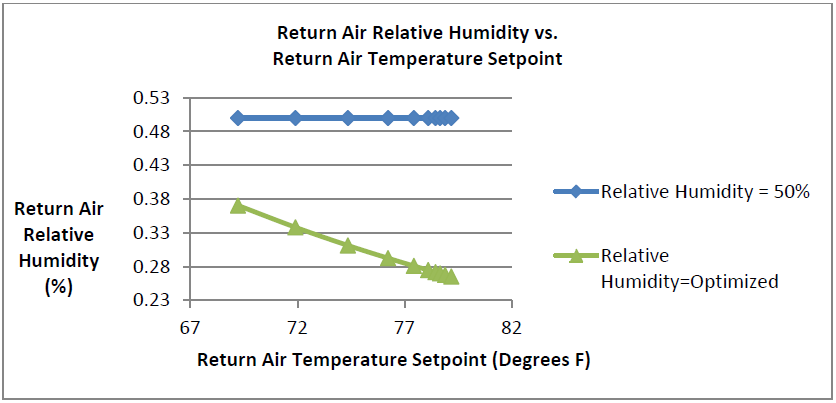
\includegraphics[width=5in]{Resources//SeeberAndSeeberHumidityEffect.png}
\caption{Graph from the paper indicating that  decreasing air relative humidity towards a lower threshold means that the air in the data centre can be warmer before it must be cooled by the \gls{CRAC} or \gls{CRAH} \cite[The Numbers: How Much Can You Really Save Through Environmental Optimization?]{SeeberAndSeeberImprovingDataCenterEnergyEfficiencyThroughEnvironmentalOptimization}.}
\label{fig:SeeberAndSeeberHumidityEffect}
\end{figure}

The trade off in the decreasing rate of prevention of hot-spots in equipment due to \gls{recirculation} at over 5000 $CFM$ \cite[The Numbers: How Much Can You Really Save Through Environmental Optimization?]{SeeberAndSeeberImprovingDataCenterEnergyEfficiencyThroughEnvironmentalOptimization}, and the increased energy consumption that increasing airflow to this rate entails can be used as a rule in the development of the \emph{logic engine} (see section \ref{sec:Methodology:TechnicalOverview:TheLogicEngine}): A way of simulating this could be to have increased airflow up to 5000 $CFM$ resulting.

The concept of \emph{leakage} could be reflected as a concept in game: it may be possible to develop a mechanic where once the user has developed their data centre, it can be tested under varying percentage leakages, testing the validity of the user's airflow considerations \cite[The Numbers: How Much Can You Really Save Through Environmental Optimization?]{SeeberAndSeeberImprovingDataCenterEnergyEfficiencyThroughEnvironmentalOptimization}.
\\

In \textbf{Analyzing End-to-End Energy Consumption for Digital Services}, \emph{Priest et al.} provide a useful demonstration of a similar concept in so far as it involves the use of a model to represent the energy consumption of a system \cite{PreistEtAlAnalysingEndToEndEnergyConsumptionForDigitalServices}. This paper is an assessment of two other studies: \textbf{A model for green design of online news media services} \cite{SchienEtAlAModelForGreenDesignOfOnlineNewsMediaServices} and \textbf{Modeling and Assessing Variability in Energy Consumption During the Use Stage of Online Multimedia Services} \cite{SchienEtAllModelingAndAssessingVariabilityInEnergyConsumptionDuringTheUseStageOfOnlineMultimediaServices}. While the system being modeled is different, and the goal is analysis rather than the production of a game, the approach is nonetheless intriguing; it would be feasible to use a similar model with heuristic rules, where input parameters are supplied as information taken about devices, environments and other factors which affect change on the \gls{data centre} environment. Furthermore, the use of a Monte Carlo algorithm for testing over many iterations could be used for such a system: many \textcolor{red}{pseudo}-randomly preconfigured \gls{data centre} designs could be generated in order to test whether the rule set for the involved device selections work as they should in order to provide a realistic a rule set as possible.

Furthermore, as \emph{A Model for Green Design of Online News Media Services} uses a principle called ``\emph{Life Cycle Assessment}" as its methodological basis, which is defined by the Global Development Research Centre define as a set of procedures used to examine the inputs and outputs in terms of materials and energy of a system, and the environmental affects directly attributable to these, assuming the ``\emph{life cycle}" to be the connected states of the system from its creation until its disposal \cite{GDRCLifeCycleAssessmentDefinition}. This approach may be a useful tool in the context of the game, as it could be developed with the overall objectives of the player being focused on achieving sustainability in terms their \gls{data centre}'s carbon footprint from a life cycle assessment perspective; it would be possible to further extend this to include such factors as the energy efficiency of disposal of and expected operational lifespan of equipment chosen in game.

\subsection{Studies into the Energy Efficiency and Cost Effectiveness of Devices and Elements of Data Centres}
\label{sec:ACriticalReviewOfReleventScientificAndEngineeringLiturature:StudiesIntoTheEnvironmentalEffectsAndEnergyEffiencyOfDataCenters}

\textbf{The Different Types Of Air Conditioning Equipment for IT Environments}  \cite{TonyEvansTheDifferentTypesOfAirConditioningEquipmentForITEnvironmentsWhitePaper} is a useful source of information on components and the rules used to model them. The paper claims that there are five distinct types of cooling systems used in \gls{data centre}s \cite[The 5 basic IT environment heat removal methods]{ TonyEvansTheDifferentTypesOfAirConditioningEquipmentForITEnvironmentsWhitePaper}.

\textcolor{red}{Below is a list of systems discussed in the study, rendered as a table for easier comparison. The advantages and disadvantages of the systems are discussed as the study discusses them:}

It is worth noting that this study does not provide supporting evidence or citations for any of the claims made about the systems. As this is a white paper, it can be assumed that this information is considered to be expert testimonial from the author, however, in the same vein, it must be considered that a salesmanship agenda may be present, attempting to attract readers to certain types of cooling system, and dissuade them from others.

\emph{Direct Expansion (DX) Air Cooled Systems}  are two piece systems that rely on warm air being drawn into a \gls{CRAC} where it comes into close proximity with a cooled and compressed fluid refrigerant, which is pumped to a fan system located outside of the \gls{data centre}, where it is able to lose heat by passing through a trough or tank with a large surface area, where it can loose heat too the air, which is drawn away by fans. In function, this system is fundamentally the same as a commercial air conditioning system \cite{ DataCenterHuddleCRACVsCRAHDefinition}.
   
Their primary advantage is that they are easier to maintain and cheaper to install than the other systems.

Their disadvantages are as follows:

\begin{itemize}
\item They are less effective at cooling larger spaces.
   
\item Pumping the refrigerant over great distances can require a lot of energy, which can negate financial savings made by installing the cheaper \emph{DX} system in the first place.
\end{itemize}

They are intended for use in small to medium sized data centres, where pumping the coolant short distances will not be as expensive.
  
\emph{Air Cooled Self Contained Systems} are single-piece systems which work by drawing air into themselves and directing it away from the \gls{data centre} as a stream of exhaust air heated to 49$^{\circ}$C, allowing for more warm air to be drawn into the system. For this to work, the air being drawn into the system must be cool and come from outside of the system, so as  to avoid warm air being drawn into the resultant vacuum\cite[Air cooled self-contained systems (1-piece)]{ TonyEvansTheDifferentTypesOfAirConditioningEquipmentForITEnvironmentsWhitePaper}.

Their primary advantage is that their installation is cheaper, and they benefit from better testing.

Their disadvantages are as follows:
\begin{itemize}
   \item Lower capacity for the removal of warm air, and the requirement of potentially expensive ductwork for the removal of warm air. 
   \item Less effective for cooling than other systems, meaning more of them may be required, which may negate their lower set-up cost.
\end{itemize} 

\newglossaryentry{hot spot}
{
  name=Hot Spot,
  description={A hot spot occurs when a data centre device such as a server rack is
  allowed to become much warmer than its surroundings.Hot spots can be the
  product of recirculation, where warm are is allowed to pass over devices that
  have not been cooled \cite{BanuelosManagingDataCentreHeatIssues}.}
}

They are best used in small data centres, or as support coolers in large \gls{data centre}s that rely on other systems for their primary cooling. Also useful for spot cooling devices that may potentially be exposed to \gls{hot spot}s.\\
 
\emph{Glycol cooled systems} use glycol (a mixture of water and ethylene glycol) as its cooling agent, which is a more efficient transfer medium for heat than water \cite{TonyEvansTheDifferentTypesOfAirConditioningEquipmentForITEnvironmentsWhitePaper}, but has a lower specific heat capacity than clean water \cite{EngineeringToolBoxEthyleneGlycolHeatTransferFluid}. Similarly to the air cooled DX system, the \emph{glycol cooled system} includes a heat exchange system inside the room to be cooled, and a fluid cooler and pump system external to the building (often roof mounted). Also similarly to the air cooled DX system, this air cooler uses forced air circulation over a coil through which the coolant flows to reject heat to the surrounding air. 

Their advantages are as follows:
\begin{itemize}
   \item The air-refrigerating section of this system is a singular self contained and factory tested unit.
   \item These can run much longer coolant pipes than air coolant systems, and that a single pump package can supply many glycol based \gls{CRAC} units on a single coolant circuit.
   \item Glycol can be cooled to -10$^{\circ}$C, meaning that an additional stage can be incorporated into the system, called ``free cooling", which involves allowing coolant to pass through an economiser coil into which air is drawn, before it reaches the refrigerator stage. In some cases, this can allow the refrigerator to be turned off, saving energy if local environmental factors allow for the fluid cooler section to be cooled to -10$^{\circ}$C.
\end{itemize}

Their disadvantages are as follows:
\begin{itemize}
   \item Because of glycol's lower specific heat capacity, this system may require a larger volume of flowing glycol than an equivalent water cooling system \cite{EngineeringToolBoxEthyleneGlycolHeatTransferFluid}. 
   \item A pump system is required for the movement of the glycol fluid, which raises installation and maintenance costs.
   \item The glycol fluid is expensive and has the potential for chemical degradation, and that an additional potentially dangerous source of liquid is introduced into the \gls{data centre} environment.
   \item The glycol mixture is toxic to humans \cite{friedmanConsequencesOfEthyleneGlycolPoisoning} and many other species \cite[8.3 Environmental risk factors]{CICAEthyleneGlycolEnvironmentalAspects}. This means that measures must be taken to prevent exposure of the glycol coolant to humans and the environment (particularly as part of the coolant circuit is external to the building), and measures to address damage caused in the event of a leak must be addressed. Both of these circumstances are potentially costly for the organisation.
\end{itemize} 

\textcolor{red}{[ADD A BEST DATACENTRE SIZE]}
   
\emph{water cooled systems} are similar in design and function to glycol cooled systems, instead using water as its flowing coolant. Rather than the external cooling coil assembly of the glycol cooled system, \emph{water cooled systems} use an assembly called a cooling tower, which sprays the warm water from the coolant circuit onto the inward-tapered sides of the tower, which are lined with a spongy material called \emph{fill}. The fill absorbs the water, which spreads through it, meaning that a greater volume of water is in contact with air at any given time. Similarly to the human sweat response, this greater exposure to air means that more water can evaporate, allowing for the overall body of water to loose heat more rapidly than if less of its surface were exposed to air \cite{exploritSweatEvaroration}\cite{healthyLivingSweatEvaporation}. Furthermore, this evaporation is aided by a fan, which draws more air through the fill, accelerating evaporation. 

Their advantages are as follows:
\begin{itemize}
   \item Condenser water from a building's existing air conditioning system can be used in this system also. 
   \item this is a fully sealed system, which, as a single unit (within the building) is factory sealed and tested. 
   \item This type of system can handle long distances of piping for the water to flow through, which means that multiple units can by connected as a circuit, potentially requiring fewer pumps than systems where several isolated cooling systems are required.
\end{itemize} 

Their disadvantages are as follows:
\begin{itemize}
   \item The "factory-sealed" aspect of this system could entail expensive maintenance by only those trained to open the unit.
   \item Long serial water coolant circuits may take on too much heat, reducing the efficiency of each cooler along the circuit.
   \item This system has a high installation cost, likely due to the specialized components involved: it is not unreasonable to a assume that the factory-sealed interior unit would come at a higher cost due to the testing and processes mentioned as an advantage of the system.
   \item Cleaning of the system as well as water treatment give this system a high maintenance cost as well. 
   \item Water will be lost from the cooling tower due to evaporation, particularly in warmer environments; therefore, the system would need to be periodically topped up with water, or potentially fully drained, cleaned and refilled, meaning that a very high cost would be incurred simply for providing the water supply for such a system.
\end{itemize}

\textcolor{red}{[ADD A BEST DATACENTRE SIZE]}
   
\emph{Chilled water systems} are similar to water cooled systems in that they involve water as their coolant, and a cooling tower of the same configuration, however, the paper claims that rather than the standard \gls{CRAC}, chilled water systems use a \gls{CRAH}; the paper describes a \gls{CRAH} as being the unit of the system which draws cool air in, but differs from \gls{CRAC} systems by drawing that air through chilled water coils.
As such, this type of system requires that water flowing through the \gls{CRAH} units be chilled, not simply cooled by the cooling tower. This chilling of the water is performed by heat-exchanging chiller unit, which allows the circuit to loose heat to a separate circuit that runs to the cooling tower. As such, this system is unique relative to the others in that it uses two separate circuits of coolant fluid. See figure \ref{ChilledWaterCRAHSystemDiagram} for an illustration of this type of system.

The advantages of this type of system are as follows:
\begin{itemize}
   \item This system's \gls{CRAH} system takes up less space in the room to be cooled than the equivalent \gls{CRAC} of any of the other systems, because a \gls{CRAH} is simply a chilled water coil and potentially a fan intake system. Components such as compressors would be located with the rest of the chiller assembly. 
   \item It follows this centralisation of the chiller system means that multiple \gls{CRAH} units can be chilled by one chiller, with all of them exchanging heat into a single coolent circuit, leading into the cooling tower circuit. The primary limitation on the number of \gls{CRAH} units connected in this isolated fashion, or in a serial configuration with the chiller would be the rate at which heat could be exchanged between the two coolant circuits.
   \item These systems have the lowest cost per kilowatt for large installations.
\end{itemize}

The disadvantages of this type of system are as follows:
\begin{itemize}
   \item This system has higher costs relative to other systems for installations below 100kW of electrical load for the facility's IT equipment.
   \item There exists a danger of introducing an additional source of liquid into the IT environment with this system, potentially leading to damage.
   \gls{CRAH} units are greater dehumidifying agents than \gls{CRAC} units, thus measures may need to be taken to humidify the room to avoid dangerous static electricity build-up in the IT equipment.
\end{itemize}

\textcolor{red}{[ADD A BEST DATACENTRE SIZE]}

\begin{figure}[H]
   \centering
   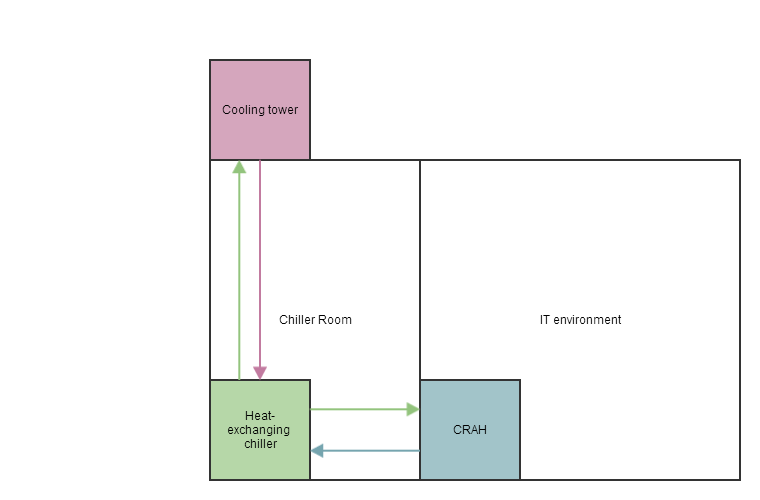
\includegraphics[width=5in]{Resources//ChilledWaterCRAHSystemDiagram.png}
   \caption{Diagram illustrating the \emph{chilled water system} configuration. Note the system has two separate coolant circuits: one between the \gls{CRAH} and the chiller, and one between the chiller and the cooling tower.}
   \label{fig:ChilledWaterCRAHSystemDiagram}
\end{figure}

As a whole, this list of different cooling system provides a good general overview into the mechanics of various types of system, however, the paper's complete lack of sources harms its credibility, and in many places assumes a knowledge greater than that of a layman, despite the theme of the paper being one of explanation of computer room cooling systems to readers not necessarily informed on the subject; a good example of this being the paper's baseless claim that \gls{CRAH} units are more dehumidifying than \gls{CRAC} units.
\\

In \textbf{PAUC: Power-Awarre Utilization Control in Distributed Real-Time Systems}, \emph{Xiaorui Wang et al.}  demonstrate that adjusting CPU usage enables distributed different distributed computing tasks to be completed depending on the environment and the task being worked on \cite{PAUCPower-AwareUtilizationControlInDistributedRealTimeSystems}.

The paper introduces that a problem with Direct Real-time Embedded (DRE) systems, when working on \emph{unpredictable tasks} or in \emph{unpredictable environments} is that it can be difficult to predict when changes to the speed required of CPUs in a distributed system will need to occur, leading to inefficient use of power with CPUs running faster than is required at certain times, or ineffective use of the CPUs themselves by running them too slowly for the task at hand.

Additionally, the paper proposes a system called \emph{Power-Aware Utilization Control (PAUC)}, a two stage regulatory system, where each processor is monitored for the speed it is running at, and the system is allowed to increase or decrease processing speed in real time according to what occurs.

The paper includes extensive testing of PAUC for controlling a group of four Linux servers, each outfitted with 2.4GHz AMD Athlon 64 3800+ CPUs and 1GB of RAM.
An immediate criticism of this method is that only the one group of machines is used: It is appreciable for the sake of elimination of anomalies stemming from using different devices the experimenters chose to operate in this way, but the test could have been repeated on a group of machines different from the first group. Furthermore, it is not unreasonable to assume that in real-world data centres, networks of differing devices with differing hardware may be used, and the experimenters could have performed a subsequent test to analyse the performance of PAUC in such scenarios.

The experimentation itself shows a how the system responds to changes in demand on one of the servers: PAUC successfully causes the CPU frequency of the test server to increase 8\% at 600ms into the test during an increase in required task processing rate. This test also shows the CPU frequency decrease back to its original value when the task rate decreases at 1200ms into the experiment, reducing power usage automatically. This shows the validity of PAUC for controlling the CPU frequency in single CPUs.

The paper concludes that PAUC, is more effective as a power and usage control solution than a system designed for a similar purpose, which is called EUCON \textcolor{red}{[NOTE: FIND THIS ANACHRONYM]}, claiming that PAUC has both greater adaptability and lower overall power consumption than EUCON. While this is true of the experiment performed, the aforementioned limitations of the experimenter's choice of experimental apparatus means that this conclusion is difficult to generalise beyond this experimental circumstance.

As shown by the study, it is possible to vary the frequency of, and by implication the power consumption of CPUs used in distributed computing systems based on the real-time tasks they are performing \cite{PAUCPower-AwareUtilizationControlInDistributedRealTimeSystems}. This indicates that PAUC could be a decent choice for automating real-time CPU usage on individual servers data centres, which is something that can be modelled as a component of the game in the Component Database, although to do this would require investigation into the effect of PAUC and similar systems with other hardware set-ups.

It is necessary to consider the positive and negative impact of potential inaccuracy of PAUC-like systems as components in-game. These costs should be weighed in terms of money saved (through kilowatt-hour average financial conversion) and the overall impact on the processing speed of the data-centre.


%\subsubsection{\textcolor{yellow}{Commercial and User Reviews of Passive Cooling Systems}}

%\textcolor{red}{[NOTE: Everything in \textcolor{yellow}{yellow} needs to be re-assessed as to whether it is to be included in the lit review.]}
%\begin{itemize}
%\item \textcolor{yellow}{\emph{bit-tech.net review of the Akasa-Euler case}: The review describes a fan-less small-footprint case, which achieves passive cooling through the CPU itself being in contact with the aluminium case, turning it into a heat-sink, meaning that no active cooling system is required, saving on construction and operating costs per unit. \cite{bit-techAskerEulerPassiveCoolingCaseReview}. The review explains that the case would require a specialised, small profile motherboard, which would be extremely restrictive for use as a server casing as only certain processors, primarily aimed at the home-PC marked would be compatible, meaning that to be used as servers in a data-center, more of them would be required, detracting from the financial saving made by the lack of requirement of a cooling system. Furthermore, the case has a limited number of connections for peripherals.}

%\textcolor{yellow}{These disadvantages, however, do not rule it out for use with on-site workstations for monitoring or administrative use.}

%\textcolor{yellow}{This article does provide a specification list, and a demonstration of why the case is unsuitable for hardware upgrading and expansion, however, it lacks comparative analysis with other similar, or indeed actively cooling devices.}
%\end{itemize}

\subsection{Studies into the Application of Artificial-Intelligence in Strategy Games}
\label{sec:ACriticalReviewOfReleventScientificAndEngineeringLiturature:StudiesIntoTheApplicationOfArtificialIntelligenceInStrategyGames}

With \textbf{Short Term Decision Making with Fuzzy Logic And Long Term Decision Making with Neural Networks In Real-Time Strategy Games},
\emph{Ert\"urk} describes AI for \emph{Real Time Strategy (RTS)} games as a hierarchy of rules which become applicable as advances in the game are made \cite[Section 3]{RTSAILogic}. He gives the example of a game where players must build and defend a village: In this scenario, one cannot train knights until a stable is built. Therefore, rules surrounding the production of knights are \emph{child} rules of rules surrounding the production of a stable.

His principle example is of the RTS \emph{Age Of Empires II}, which he describes as suffering from the limitation of exclusively using rule-based AI for the management of the computer-controlled player: This made it possible to predict the actions of the computer-controlled player as it can never overcome the limitations of it's knowledge-base.

%While this source is taken from the author's on-line blog, it is well written, detailing the subject in a scientific manner, whilst using terminology that allows the layperson to read it. The section reviewed does not appear to directly cite any sources for its information, although the article does appear to link to other sources for more information. This does somewhat detract from the reliability of the section.

The limitations Ert\"urk \cite[Section 3]{RTSAILogic} describes for the rule-based AI of \emph{Age Of Empires II} are not necessarily as relevant to the game application developed in this project: \emph{Age Of Empires II} is described as being a war game, taking place on outdoor battlefields, a scenario that is much more dynamic than that of a data centre, and may require more rules in order to model it: The \gls{data centre} scenario necessitates rules such as temperature restrictions, financial restrictions and interactions between components, rather than the navigation of decision engines within a two dimensional space. Therefore, it is the authors opinion that these drawbacks do not apply as readily to the game being developed, but should be considered during development in order to avoid AI issues.

Er\"turk's described hierarchical structure would be an interesting model to use in the game, as it would allow new rules to be implemented as new components are added in-game.

\subsection{Observations and studies of browser-games developed using JavaScript}
\label{sec:ACriticalReviewOfReleventScientificAndEngineeringLiturature:ObservationsAndStudiesOfBrowserGamesDevelopedUsingJavaScript}

\textbf{Unreal Engine 3, Ported to JavaScript} is an impressive demonstration of what is possible using JavaScript is a browser game and technology demonstration called Epic Citadel \cite{EpicCitadel}, which features a fully three-dimensionally rendered medieval town which can be explored by the user. This game utilises Epic Games' Unreal Engine 3 ported to JavaScript, and able to run in any JavaScript compatible web browser, as long as the user's system is capable of handling the system requirements of the game.

The technology was reviewed by Grant Brunner \cite{Unreal3JavaScriptExtremeTech}. The article praises the technical achievement that this represents, and the speed at which it was developed, hailing it as potentially representing a future of cross-platform 3D games which need only be coded once without the need to port to other languages or clients.
The article does suggest that playing Epic Citadel will crash users' browsers, precluding them from actually testing the game themselves. Unfortunately, this does make their claims about the technology appear conjectural at best.

This technology demonstration itself is impressive, and displays what is possible using JavaScript programming embedded into websites. This demonstrates that the development of a 3D GUI for the game is a potentially viable option.

\newglossaryentry{third-person}
{
	name=Third-Person,
	description={In the context of 3D gaming, a \emph{third-person} game is one where the gamer's view is from a position external to any character in the game world, where they are generally not interacted with. As such, a full view of the character which the gamer is controlling is generally visible, with that character being the gamer's means of interacting with the game environment}
}

\newglossaryentry{first-person shooter}
{
	name=First-Person Shooter,
	description={A genre of game where the player's view of the game environment is through the eyes of the character they are playing as. As such, the player's interactions with the game world are directed towards themselves. As shooters, these games generally involve combat using firearms, or similar styles of directed (often ranged) combat.}
}

During the 2014 mloc.js conference, \emph{David Galeano} gave a presentation entitled \textbf{JavaScript and the browser as a platform for game development}, in which he discusses \textbf{\emph{Turbulenz}}, which is both a JavaScript based game engine usable for both 2D and 3D games, and the name of the company that produces it \cite{GaleanoJavaScriptForGameDevelopment}. During this, \emph{Galeano} demonstrates two browser based games which have been developed entirely using JavaScript: \emph{Polycraft} \cite{Polycraft}, which is a 3D \gls{third-person} ``persistent floating island game", and a demo of the popular \gls{first-person shooter} game \emph{Quake 4}.

The Turbulenz implementation of Quake 4 is not intended by Turbulenz to be a full game, but rather a demonstration that the Turbulenz engine can be used to support a version of the game which is visually simmilar to the original game, which is based on the C++ coded \emph{id-tech 4} engine used for the native version of Quake 4 \cite{ModDBIdTech4Download} \textcolor{red}{[ADD A CITATION TO SAY THAT QUAKE 4 USES ID TECH 4]}. As such, rather than a coherent demonstration of game-play following a traditional plot, the demonstration is used to show that conventional \gls{first-person shooter} features such as weapons usage and animation, 3D graphics, animation of characters, and shading and lighting of the environment and objects with in it relative to ambient and spot light sources can be achieved on this JavaScript based platform.
Furthermore, in the YouTube video entitled \textbf{Turbulenz WebGL Engine using Quake 4 assets}, \emph{Galeano} demonstrates the Turbulenz JavaScript port of Quake 4 assets, whilst also discussing some of the technicalities of how porting a game such as Quake 4 as a browser game can be achieved \cite{TurbulenzWebGLQuake4AssetsVideo}. Turbulenz uses WebGL to render graphics, and \textcolor{red}{WebAudio} for sound. WebGL seems to be a solid choice for this, because this game features many assets, including three dimensional objects and rooms, various surface textures, as well as rooms containing as many as thirty light sources rendered in real time (as demonstrated by rotating spot lights \cite{TurbulenzWebGLQuake4AssetsVideo}), thus demonstrating that it is entirely possible to develop a complex three dimensional game environment in JavaScript.

In the conference,\emph{Galeano} discusses a few of the issues which currently impose a performance gap between browser games, and native games \cite{GaleanoJavaScriptForGameDevelopment}. They are as follows:

\begin{itemize}
	\item \emph{Memory usage}, with the memory requirement overhead being higher than standard JavaScript objects can handle, which can lead to cache errors, and difficulty maintaining storage of objects in arrays. \textcolor{red}{Presumably, this high memory requirement may also lead to issues arising due to the browser game being further abstracted from system resources than a native game would be.}
	
	\item \emph{Parallelism} for games on the Turbulenz engine is not currently available; \emph{Galeano} states that drastic improvements would be possible if it were to become possible for a JavaScript based browser game to take advantage of more than the single core available to the browser in systems with more than a single CPU core available.
	
	\item \emph{64-bit floating point operations} (e.g. ``double precision" operations) are a requirement of standard JavaScript operations, however, \emph{Galeano} claims that in most games, \emph{32-bit floating operations} offer greater speed, with an acceptable drop in accuracy of operations such as graphical rendering. This raises a conundrum: While it is possible to make a JavaScript compiler use 32-bit floating point operations where 64-bit precision is not required, Turbulenz already features a great deal of code written that does not take advantage of such a system, so it is impractical to modify it in this way. As such, \emph{Galeano} states that it would be an advantage to the Turbulenz if an update to JavaScript were made that would allow Turbulenz to be compiled in its present form, but allowing it to select 32-bit floating point operations where it is able to do so.
\end{itemize} 

\textcolor{red}{[FIND OUT IF YOU NEED TO CITE THE MP3 OF THE CONFERENCE, OR IF THE .PDF ALONE COUNTS]}

In \emph{Turbulenz WebGL Engine using Quake 4 assets}, \emph{Galeano} states that the Turbulenz uses the \textbf{WebGL} JavaScript API for rendering 3D graphics \cite{TurbulenzWebGLQuake4AssetsVideo}. \emph{Gregg Tavares} defines WebGL as being a 2D graphics API which is capable of rendering 3D graphics in real time\cite{WebGLFundamentals}. This article explains that WebGL uses two shaders to draw onto a HTML5 canvas page element:

\begin{itemize}
\item A \emph{Vertex shader}, which takes clipspace co-ordinates. These co-ordinates represent a position on the canvas ranging from \textcolor{red}{\textsuperscript{-}1 to \textsuperscript{+}1}, and are given as a pair of values; X axis (vertical) position and Y axis (horizontal) position. For example, \url{0,0} would represent the bottom left hand corner of the canvas, \url{1,1} the top right, and \url{1,0.5} the centre of the right-hand edge. This clipspace based system has the advantage of automatically scaling to fit the display it is being presented on, not matter its size, because the pixels available for the canvas will be divided into a \textcolor{red}{\textsuperscript{-}1 to \textsuperscript{+}}1 clipspace continuum.

\textcolor{red}{[IT SAYS IN HERE +1 TO -1, BUT EXAMPLES ARE 0 TO 1. FIND OUT WHY THIS IS]}

\item A \emph{fragment shader}, which provides colour.
\end{itemize} 

\textcolor{blue}{The article says that the same principle is used when drawing images as textures with WebGL; The coordinates form where the image is drawn to where it ends are supplied to the vertex shader, while the image \textcolor{red}{file} itself us supplied to the fragment shader, in order to get the colours necessary to render it, before the image itself is copied to the position on page using these properties \cite{WebGLFundamentals}.}

\textcolor{red}{The article states that in order to reproduce 3D graphics, shaders which convert a 3D model into a 2D image must be supplied.} Often, third party libraries must be used to do this, such as \textbf{three.js} \textcolor{purple}{\cite{three.jsManual}} and \textbf{GLGE} \textcolor{purple}{\cite{GLGEWebsite}}. Both of these libraries provide support for 3D animation, directional lighting, skeletal animation, shadows, and other features expected of modern 3D computer graphics. In order to develop the Turbulenz version of the Quake 4 engine using WebGL \cite{TurbulenzWebGLQuake4AssetsVideo}, \emph{Galeano} must have used one of these libraries, or a simmilar JavaScript library in order to make Turbulenz able to render real-time 3D graphics in the way that it does. \textcolor{purple}{[NOTE: THE LINKS IN PURPLE ARE PRIMARY SOURCES- MAKE SURE IT IS OKAY TO USE THESE.]}

\textcolor{red}{[NOTE: CONSIDER INCLUDING STUFF RESEARCHED FROM \cite{WebGLUpAndRunningTonyParisi}]}
% ------------------------------------------------------------------------
% -*-TeX-*- -*-Hard-*- Smart Wrapping
% ------------------------------------------------------------------------
\def\baselinestretch{1}

\chapter{Development}
\label{chapter:Development}

\def\baselinestretch{1.66}


%%% ----------------------------------------------------------------------

This chapter chronicles the development of the application, as well as testing of each individual element of the project as it is developed, in order to further refine it. This testing should not be confused with the testing section (chapter \ref{chapter:Testing}), which is larger scale testing of interactivity between system components, and of the system as a whole.

%%% ----------------------------------------------------------------------
\goodbreak

\section{Investigations}
\label{sec:Investigations}
This section chronicals experimentation undertaken to develop skills and basic \textcolor{red}{frameworks} using technologies identified as being useful to the project.

At the end of each of these sections, a series of aspects which will be included in the main project are outlined.

\subsection{Java and JSON}
\label{subSec:Java and JSON}
The goal of this investigation was to find a way that a Java back-end could be integrated with a 3D JavaScript based front-end which primarily uses three.js. \textcolor{red}{[SAY MORE ABOUT THIS]}

\subsubsection{17/12/2014: Version 1 \textcolor{red}{[READ THROUGH EACH VERSION, I THINK THERE IS A LOT OF REPETITION]}}
\label{subSubSection:Java and JSON: Lab 1}
This version establishes the use of csv files as storage of data about in-game elements. A test example, servers, is used, with servers.csv (in root/resources/data).

A java class was created for the retrieval of individual rows from servers.csv; ServerDataRetriever.java, which retrieves rows based on a supplied "key" string; All rows from the file are added to an array list, which is checked through iteratively using a for loop, which limited by the size of the array list: if a row string containing the key string is found in the array list, it is assigned as the output of the class's .getRow() method. 
ServerDataRetriever.java retrieves servers.csv's file path by getting its own runtime file path from the class loader, which it converts to a character array, removes all elements of it that do not correspond to the root of the application folder, and finally converts it to a string and concatenates the rest of the file path to it. 
Specifically, it does this adding all characters to the character array, then adding all but the last 26 of them to the file path string, with 26 being a known quantity of characters beyond the root folder in the class loader pathway for this file at run time.

For testing purposes, a server with the name (and key) "Type1" is retrieved, and is displayed on General\textunderscore MainPage.jsp as a java bean. As such, no JavaScript is used in this version because this version is intended only as a test of CSV files for data storage, and retrieval of data from them as rows.

\subsubsection{21/12/2014: Version 2}
\label{subSubSection:Java and JSON: Lab 2}
ServerRetriever was modified and renamed DataRetriever. Specifically, the getRow was modified to take one more string parameter, fileName, which is used to determine which file within the data folder to search for the specified row. This means that the one class can now be used to search any CSV file in the folder. 
DataRetriever was modified to retrieve a newly added header row from the CSV files using method ArrayList getHeaders(), which adds these as individual strings using a for loop and an if statement which iterates through the header row as a character array, concatenating characters to a string, which is added to the output array list whenever a comma is encountered in a character array. 
getHeaders is called from another new method, String convertToJSON(String), which itself is called by String getRow(). The method convertToJSON takes the row retrieved by getRow, adds it's CSV elements to an ArrayList in the same way that getHeaders does with the header row, and concatenates these elements with those returned by getHeaders into a JSON format string, where headers are assigned to values. 

DataRetriever's pathway assignment was abstracted to a string returned by a class called DataFolderFilePathPointer.java, which is a smaller class with a final string containing the absolute resources/data pathway for the system being used, allowing for easier set up of the project on different systems. 

As a test of the JSON value being retrieved, it is called as a java bean into \url{General_MainPage.jsp}, where it is called to be displayed on page in a pargraph with the id value "demo", having been parsed as a JSON object, with each element being called by it's respective header values, e.g. once added and JSONified, server "Type1" is called as obj.name.

\subsubsection{21/12/2014: Version 3}
\label{subSubSection:Java and JSON: Lab 3}
ServerRetriever was modified and renamed DataRetriever. Specifically, the getRow was modified to take one more string parameter, fileName, which is used to determine which file within the data folder to search for the specified row. This means that the one class can now be used to search any CSV file in the folder. 
DataRetriever was modified to retrieve a newly added header row from the CSV files using method ArrayList getHeaders(), which adds these as individual strings using a for loop and an if statement which iterates through the header row as a character array, concatenating characters to a string, which is added to the output array list whenever a comma is encountered in a character array. 
getHeaders is called from another new method, String convertToJSON(String), which itself is called by String getRow(). The method convertToJSON takes the row retrieved by getRow, adds it's CSV elements to an ArrayList in the same way that getHeaders does with the header row, and concatenates these elements with those returned by getHeaders into a JSON format string, where headers are assigned to values. 

DataRetriever's pathway assignment was abstracted to a string returned by a class called DataFolderFilePathPointer.java, which is a smaller class with a final string containing the absolute resources/data pathway for the system being used, allowing for easier set up of the project on different systems. 
Furthermore, DataRetriever's getRows and getHeaders methods were modified by having the strings where characters from their character arrays added to their respective string ArrayList objects, which overcame a bug where the last column header and row attribute were not being added to the JSON formatted string. 

For this version, \url{General_Mainpage.jsp} requests an entry from "servers.csv" with the name attribute "Type1". It retrieves it by using the getRows method of an object of class DataRetriever. 
This data is processed in the following way:

It is converted from a CSV row to a JSON format string by DataRetriever.
in seperate instances, the JSON format string is converted to a JSON object by the functions addToLocalStorage and processServer of JavaScript file JSTest.js.
In seperate instances, the JSON object is displayed on page by processServer, and retrieved from LocalStorage and displayed on page by function getRowFromStorage of JSTest.js ussing jQuery append functions.
In order to test the whole process of retrieving the row, converting it to JSON format, adding it to LocalStorage and retrieving it to the page from LocalStorage, three instances of the row are displayed on-page on \url{General_MainPage.jsp}: A Java scriptlet directly displaying the raw output of DataRetriever.getRow, the converted JSON object elements displayed by function processServer, and the JSON object retrieved from LocalStorage displayed by function getRowFromStorage.

\textbf{Page list:}
\begin{itemize}
\item \url{General_MainPage.jsp}\newline
In this version, this page contains on-page JavaScript which parses the returned string from DataRetriever.getRow as JSON, and displays its content on page.\newline

 This page references the following files:
\begin{itemize}
\item \textbf{Java classes and their methods:}

\begin{itemize}

\item \url{DataRetriever.java}

\begin{itemize}

\item \url{String}  \url{getRow(HttpServletRequest, HttpServletResponse, String, String)}\newline
Adds all rows from specified CSV file to an ArrayList, checks all entries in that ArrayList for a row with which contains the String parameter (the key), outputting such a row if it is found. This method finishes by calling the method convertToJSON.

\item \url{String} \url{convertToJSON(String)}\newline 
Adds all comma-seperated elements from the row, and uses a for loop and if statement to add all of the elements in that row to an array list by iteratively checking for commas in the input string as a character array, concatenating them to a string if a comma is not found, and adding that string to a string array if a comma is found. Next, this method calls the method getHeaders, and uses its String ArrayList content to form the row into a JSON format string.

\item \url{String} \url{getHeaders()}\newline 
This uses the same iterative for loop and if statement technique as convertToJSON to get all of the CSV format elements of the first row (the column headers) of the CSV file, which are used in convertToJSON to convert its string input to JSON format.

\end{itemize}

\item \url{DataFolderFilePathPointer}

\begin{itemize}
\item \url{String} \url{getPathway()}\newline
This returns the final string filePath, which is assigned by as the pathway to the web application's resources/data folder, which is called by classes which require this, such as DataRetriever.
\end{itemize}

\end{itemize}

\item \textbf{JavaScript files and their functions:}

\begin{itemize}

\item \url{JSTest}

\begin{itemize}

\item \url{processServer(row)}\newline
Takes a JSON format string (row) as its parameter (the output of DataRetriever.getRow()), which it converts to a JSON object, and retrieves elements with the JSON name tags "name", "x", "y", and "z", appending them to the "main" div of the page using the jQuery .append() method.

\item \url{processServerOnPage(row)}\newline
Works in the same way as processServer, appending the JSON elements as a string into div "demo" using document.getElementById("demo").innerHTML.

\item \url{addToLocalStorage(row)}\newline
Works in the same way as processServer, but adds the JSON elements to LocalStorage.

\item \url{getRowFromStorage(row)}\newline
Relies on addToLocalStorage, using the jQuery function .append() to add content from LocalStorage to the "main" div.
\end{itemize}
\end{itemize}
\end{itemize}
\end{itemize}

\subsection{Design decisions stemming from this investigation}
\label{subSec: Java and JSON: Design decisions stemming from this investigation}

The following decisions regarding the server-side Java conversion of data from CSV tables to JSON objects were made as a result of these investigations:

\begin{itemize}
\item JSON appears to be a data-interchange format which is particularly easy to handle client-side using reasonably simple JavaScript, and parsing data into JSON objects server side using Java objects is also relatively straightforward, therefore, JSON will be used in the project for the purpose of passing data from the server to the client.

\item Subsequent research has found that the current design of \url{General_MainPage.jsp} will not work when wrapped for mobile with PhoneGap because PhoneGap and Cordova cannot interpret Java Server Page files. However, PhoneGap can wrap all standard HTML5 file types (HTML, CSS and JavaScript), and it does allow for the passage of XML and JSON data between the server and the wrapped site. Therefore, the classes developed could still be used, but packaged into Java servlets called by HTML pages, rather than as JSP files \cite{PhoneGap:FAQs}. \textcolor{red}{[CITE PHONEGAP IN LIT REVIEW]}
\end{itemize}

\subsection{Three.js}
\label{subSec:Three.js}
This is a log of experiments using Three.js, with a mind to integrating the technology into the project, and including a 3D interface. The project is divided into a series of labs, which chronicle the changes made by session.

\subsubsection{Lab 1: 28/12/2015: First Three.js experiment}
\label{subSubSec:ThreeJSExperiments:Lab1}
his is a very simple HTML file displaying a rotating cube. It is a excercise in the basics of using Three.js for WebGL.

\subsubsection{Lab 2: 30/12/2014: .Obj file loader test: Local library access}
\label{subSubSec:ThreeJSExperiments:Lab2}
The first stage of this lab was to reverse engineer JavaScript data found associated with the Three.js OBJLoader demonstration \cite{ThreeJSObjLoader}, which features use of OBJLoader.js; part of the Three.js library which allows for the importation of .OBJ files for display through JavaScript.

This JavaScript file first copied and tested by changing the .OBJ file link from the one within the Three.js library specified in the demo for a model of a car uploaded by a user of tf3dm.com \cite{LarsenBMWObj}, and re-skinned with a plain white texture.

\subsubsection{Lab 3: 06/01/2015: .Obj file loader test: Remote library access \textcolor{red}{[REMOVE THIS, YOU'LL BE USING GIT]}}
\label{subSubSec:ThreeJSExperiments:Lab3}
A repeat of lab 2, attempting to reference the Three.js library from its location online, rather than locally

Unfortunatly, attempts to access the files as online resources through http://cdnjs.com/libraries/three.js/, my dropbox account and github all failed. As such, the large local three.js library and this project will be relocated as part of the DataCentreModelling project, in order to conserve space.

\subsubsection{Lab 4: 06/01/2015: Object animation tutorial}
\label{subSubSec:ThreeJSExperiments:Lab4}
Following of a tutorial at Tuts+ Code Tutorials \cite{Tuts+ThreeJS} to develop an animated cube object, without the need to import an external .obj file into the project.

\subsubsection{Lab 5: 08/01/2015: Camera animation tutorial modification}
\label{subSubSec:ThreeJSExperiments:Lab5}
Lab 4 is repeated, animating the camera to spin on it's Y axis, rather than the cube object.

\subsubsection{Lab 6: 12/01/2015: TrackballControl.js: A development of the page \newline``WebGL With Three.js: Basics"} 
\label{subSubSec:ThreeJSExperiments:Lab6}
A modification of the same Tuts+ Code Tutorial used in Lab 4 \cite{Tuts+ThreeJS}, exchanging pyramids for cubes.

This experiment is undertaken to explore the potential of TrackballControls.js within the Three.js library

This was tested both on a Windows 7 system, and an Android tablet. The windows testing revealed that clicking and dragging on any part of the page would pan the camera around the scene, and using the mouse-wheel would zoom the camera into the scene (forward for zooming in, backward for zooming out). The testing on the Android tablet revealed that touching and dragging on the page rotated the camera around the scene, pinching outwards with two fingers zoomed the camera out from the scene, pinching inwards with two fingers zoomed the camera into the scene, and dragging two fingers across the screen moved the camera along an axis relative to the 3D object.

\subsubsection{Lab 7: 12/01/2015: A single lit object viewed by a trackball controlled camera}
\label{subSubSec:ThreeJSExperiments:Lab7}
A development of the work in Lab 4 (and by extention http://code.tutsplus.com/tutorials/webgl-with-threejs-basics--net-35688), producing more of a blank canvas, with the ultimate goal of producing a template JavaScript file (or collection of files) to use in the DataCentreModelling project.

\subsubsection{Lab 8: 14/01/2015: A single lit, animated object viewed by a trackball controlled camera}
\label{subSubSec:ThreeJSExperiments:Lab8}
This features an .obj 3D object file imported into the scene using an OBJLoader class object, coloured with a plain white JPEG file, and illuminated from one side by a red spotlight. The scene is also observed by a camera controlled by a TrackBallConrols class object, allowing free movement, rotation and zooming of the camera relative to the scene.

\subsubsection{Lab 9: 15/01/2015: Lighting experiment}
\label{subSubSec:ThreeJSExperiment:Lab9}
An attempt was made to produce variable colour and three.js spotlights, controlled by HTML buttons linked to embedded JavaScript was made. This failed, and was postponed due to not being essential to the project.

\subsubsection{Lab 10: 21/01/2015: Implementation of three.js voxel painter at ``three.js webgl - interactive - voxel painter"}
\label{subSubSec:ThreeJSExperiments:Lab10}
This is an implementation of source code found at a Three.js demonstration, which displays a three.js based voxel painting canvas \cite{ThreeJSVoxelPainter}.

This implements the use of "voxels", or volumetric pixels, which are added as coloured cubes to a three dimensional grid plane. This makes an interesting potential basis for the data centre modelling application: This grid-plane system could be used, with the voxels replaced by 3D objects representing items being added to the data centre floor.

\subsubsection{Lab 11: 24/01/2015: Combination of three.js voxel painter with TrackballCamera.js}
\label{subSubSec:ThreeJSExperiments:Lab11}
This experiment brings together two different projects, Lab 7 (and by extension the three.js voxel painter demonstration \cite{ThreeJSVoxelPainter}), producing a 3D voxel painter, using a three.js roll-over mesh, a roll-over helper when the cursor passes over the mesh, and allowing a black 3D cube to be placed wherever the roll-over helper is when the mouse is clicked, and for the camera to be moved around the scene by the by clicking and dragging the cursor, making for intuitive control of the voxel painter, including camera relocation.

\subsubsection{Lab 12: 04/03/2015: Inclusion of 3D objects generated from JSON files into Lab-11}
\label{subSubSec:ThreeJSExperiments:Lab12}
This is a development of lab-11, replacing the Three.js BoxGeometry cubes placed on the grid with a 3D object imported from an external file, as was the case with lab-8 and before.

Unlike lab-8, the file used to generate the 3D cones placed by clicking on the grid is a JSON file rather than an .obj file; this is because it was found to be difficult to sucessfully cast the three.js .obj file loader class object, OBJLoader, into the framework that already existed in lab-11, where as the class which interprets JSON files as 3D objects, JSONLoader, is possible to integrate in the existing manner that BoxGeometry was.

\subsubsection{Lab 13: 05/03/2015: Decomposition of ThreeJSExperiments\textunderscore Lab12.js into an object-oriented structure}
\label{subSubSec:ThreeJSExperiments:Lab13}
This is a deelopment of lab-12, decomposing it into a single JavaScript file which call various JavaScript classes, each of which is contained within it's own JavaScript file. These classes each encapsulate a single aspect of the model, for example, RolloverCursor handles the drawing of the rollover cursor cube, and Skybox handles the drawing of the skybox.

Essentially, the classes are functions, and their operations are nested functions, while importation of functions into the namespace is handled as JavaScript inclusions within the HTML document calling them. The static context from which objects of these classes are constructed, and their operations are called is the un-encapsulated part at the beginning of the calling class (henceforth the main class, which in this context is ThreeJSExperiments Lab13.js. This idea follows from the tutorial at Scorchsoft.com \cite{ScorchSoftJavaScriptObjectOrientation}.

This lab includes a number of commits to a GIT repository, outlined below:

\begin{enumerate}
\item \textbf{07/03/2015: Commit ID a1ba56d:} Created the folder web/js/lab13 as a container for experimental changes to ThreeJSExperiments\textunderscore Lab12.js, which are then added to web/js/ThreeJSExperiments\textunderscore Lab13.js. ThreeJSExperiments \textunderscore Lab13a was created, which features all of the functionality required to draw the grid-plain decomposed into function draw of pseudo-class Grid. This approach to object-oriented programming in JavaScript was found at Scorchsoft.com \cite{ScorchSoftJavaScriptObjectOrientation}.

\item \textbf{07/03/2015: Commit ID aa241ba:} Further extended pseudo-class Grid within ThreeJSExperiments\textunderscore Lab13a.js with a constructor which is called by default, and commented-out code for private and public attributes.

\item \textbf{07/03/2015: Commit ID 7c758e2:} web/js/ThreeJSExperiments\textunderscore Lab13a.js is completed; all model-level architectural elements have been decomposed into pseudo-classes, with "draw" functions for their respective elements.

\item \textbf{07/03/2015: Commit ID 14f4e84:} The class CameraControls, which was formerly part of web/js/lab13/ThreeJSExperiments\textunderscore Lab13a.js, was migrated into it's own file at web/js/lab13/model/CameraControls.js, and is successfully called from web/js/lab13/ThreeJSExperiments\textunderscore Lab13b.js, which means that camera controls are handled by that class in that file when called as \newline var cam = new CameraControls(). The class CameraControls contains a constructor, which, in the context of JavaScript deployed in this manner, is a child-function which is called within the parent function (the class itself). This means that the object is fully initialised on construction.

\item \textbf{08/03/2015: Commit ID 6dc2c35:} All code from web/js/lab13/ThreeJSExperiments\textunderscore Lab13b.js was migrated into web/js/ThreeJSExperiments\textunderscore Lab13.js, The model folder containing the model JavaScript files was migrated to web/js, and ThreeJSExperiments\textunderscore Lab13.html was modified to reference web/js/ThreeJSExperiments\textunderscore Lab13.js and the JavaScript files within the newly migrated model folder.

\end{enumerate}

\subsection{Design decisions stemming from this investigation}
\label{subSec: Three.js: Design decisions stemming from this investigation}

The following decisions regarding the front-end JavaScript 3D model interface were made as a result of these investigations:

\begin{itemize}
\item Imported three-dimensional models would be used, drawn from external data files. JSON format object files were chosen over .obj format files due to their being natively supported by the three.js library, and thus easier to parse, and because utilities exist which can convert .obj files to JSON files, such as Obj\textunderscore To\textunderscore ThreeJS \cite{ObjToJSON}.

\item The class of three.js, TrackballContols.js, will be used for camera positioning.

\item The layout as seen in Three.js - interactive voxel painter \cite{ThreeJSVoxelPainter} will be used, consisting of a two dimentional plane \textcolor{red}{superimposed over an invisible placement plane}, where a cursor can move, which allows for the placement of three dimentional objects.

\item The basic layout will involve a point-and-click interface, which will allow the user to place objects, and alter camera orientation with mouse or touch-screen gestures. 
\end{itemize}

\section{Design}
\label{sec:Design}

\subsection{JavaScript 3D front-end}

The 3D user interface was developed using WebGL via JavaScript, using the three.js library as outlined in section \ref{subSec:Three.js}. Specifically, all unique funtional requirements for the operation of the 3D modelling aspect of the web-application were identified and isolated from the JavaScript classes originally produced in section \ref{subSubSec:ThreeJSExperiments:Lab13}, further decomposing and encapsulating the functionality into more, smaller classes. This part of the project follows it's own Model-View-Controller (MVC) structure, as illustrated in figure \ref{fig:JavaScriptArchitectureDiagram}.

\begin{figure}[H]
\centering
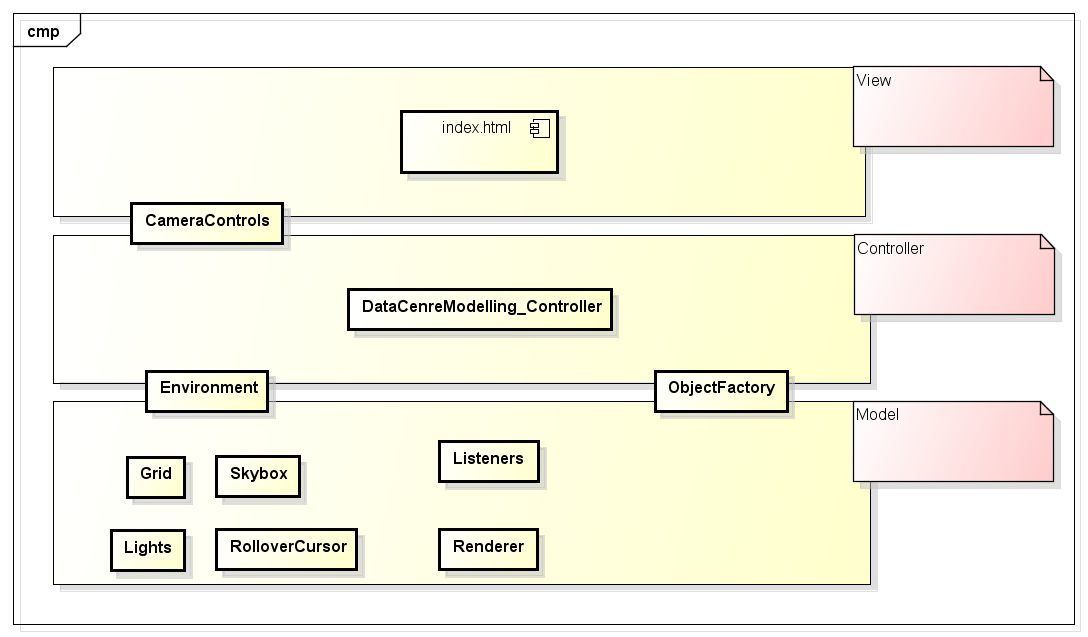
\includegraphics[width=5in]{Resources//Design_Diagrams//Component_JavaScript 3D model.png}
\caption{MVC architectural diagram of the JavaScript 3D viewer.}
\label{fig:JavaScriptArchitectureDiagram}
\end{figure}

Structurally, these classes follow a facade design pattern, with the controller class, DataCentreModelling\_Controller creating and calling the generateEnvironment method of model class Environment within it's own  method init, which is called on DataCentreModelling\_Controller's construction. 

Each one of these classes is contained within a single JavaScript file, in order to make them more intelligible to human readers, and more familiar to object-oriented programmers.

\textcolor{green}{
The classes Environment, Environment's subordinate classes, and ObjectFactory all contain constructors and encapsulated methods, functioning in much the same way as classes of any object oriented language, where as DataCentreModelling\_Controller behaves more like a static class; all of it's attributes are static, and many of them are accessed by other classes as static variables. This is nessecary to allow for certain things to occur by default, such as DataCentreModelling\_Controller's method init. This also allows for certain variables not to need to be re-assigned within subordinate classes, as attempts to treat them in that manner had failed.
[YOU GOT THIS FAR!!!]}

\begin{figure}[H]
\centering
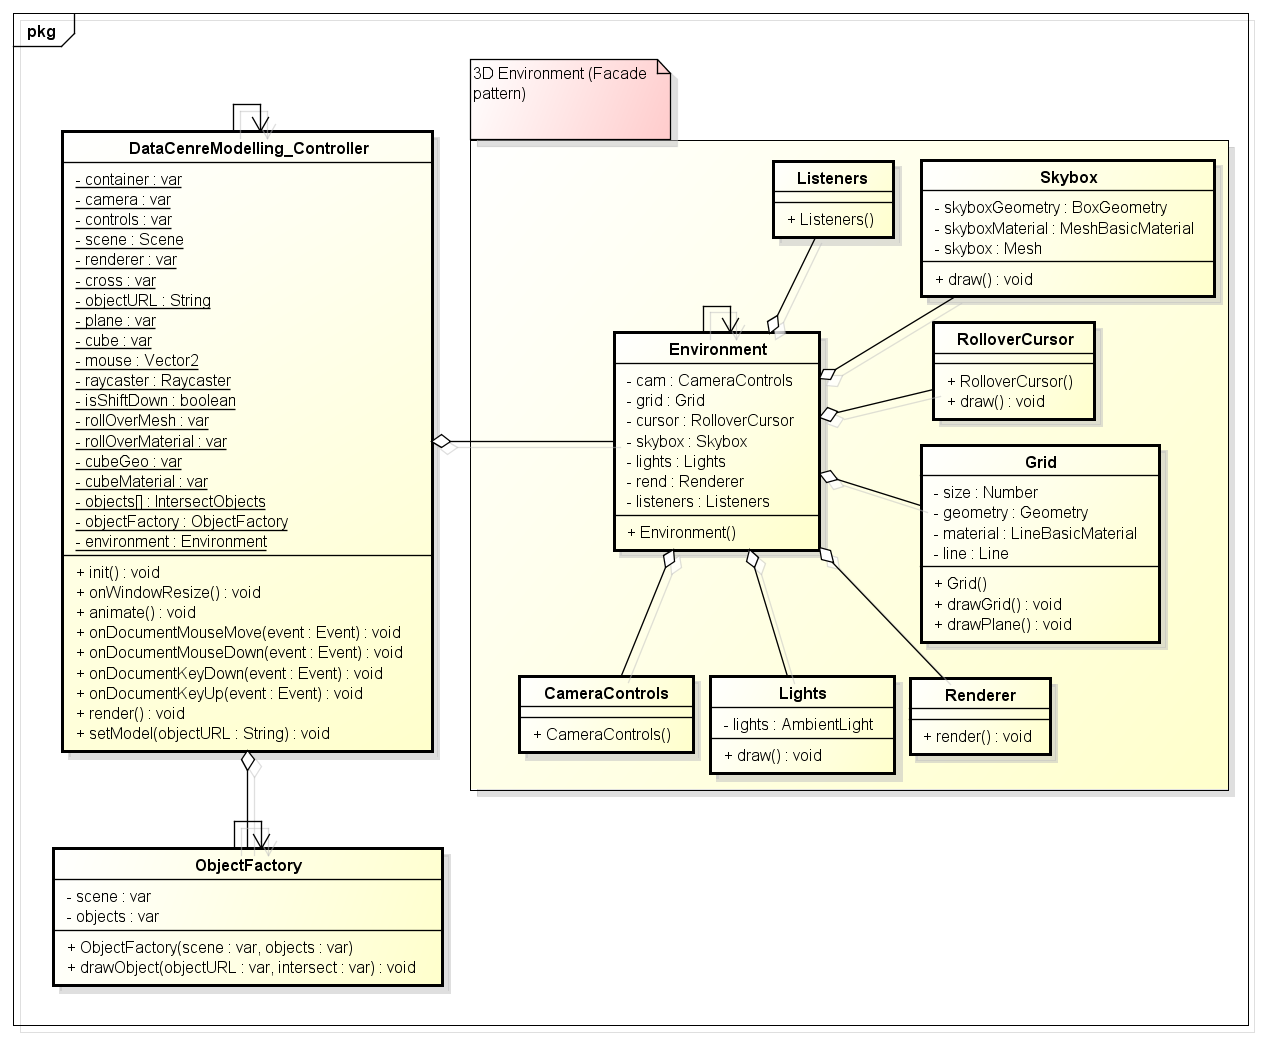
\includegraphics[width=5in]{Resources//Design_Diagrams//Class_ JavaScript Front-end.png}
\caption{UML Class diagram of the JavaScript 3D viewer. Note that due to JavaScriptbeing a weakly typed language, some attributes are labeled 'var', denoting that they are weakly typed variables. However, where a variable would have a strongly-typed analogue, such as String or into, it is labeled as such to clarify it's role. Furthermore, Where a variable is assigned as an object, even if it is not assigned that variable upon construction, is labeled as being an object of that class in order to distinguish it.}
\label{}
\end{figure}

Environment's generateEnvironment method creates objects of other classes required to generate the 3D environment, such as the grid plane, and the lights.

\begin{figure}[H]
\centering
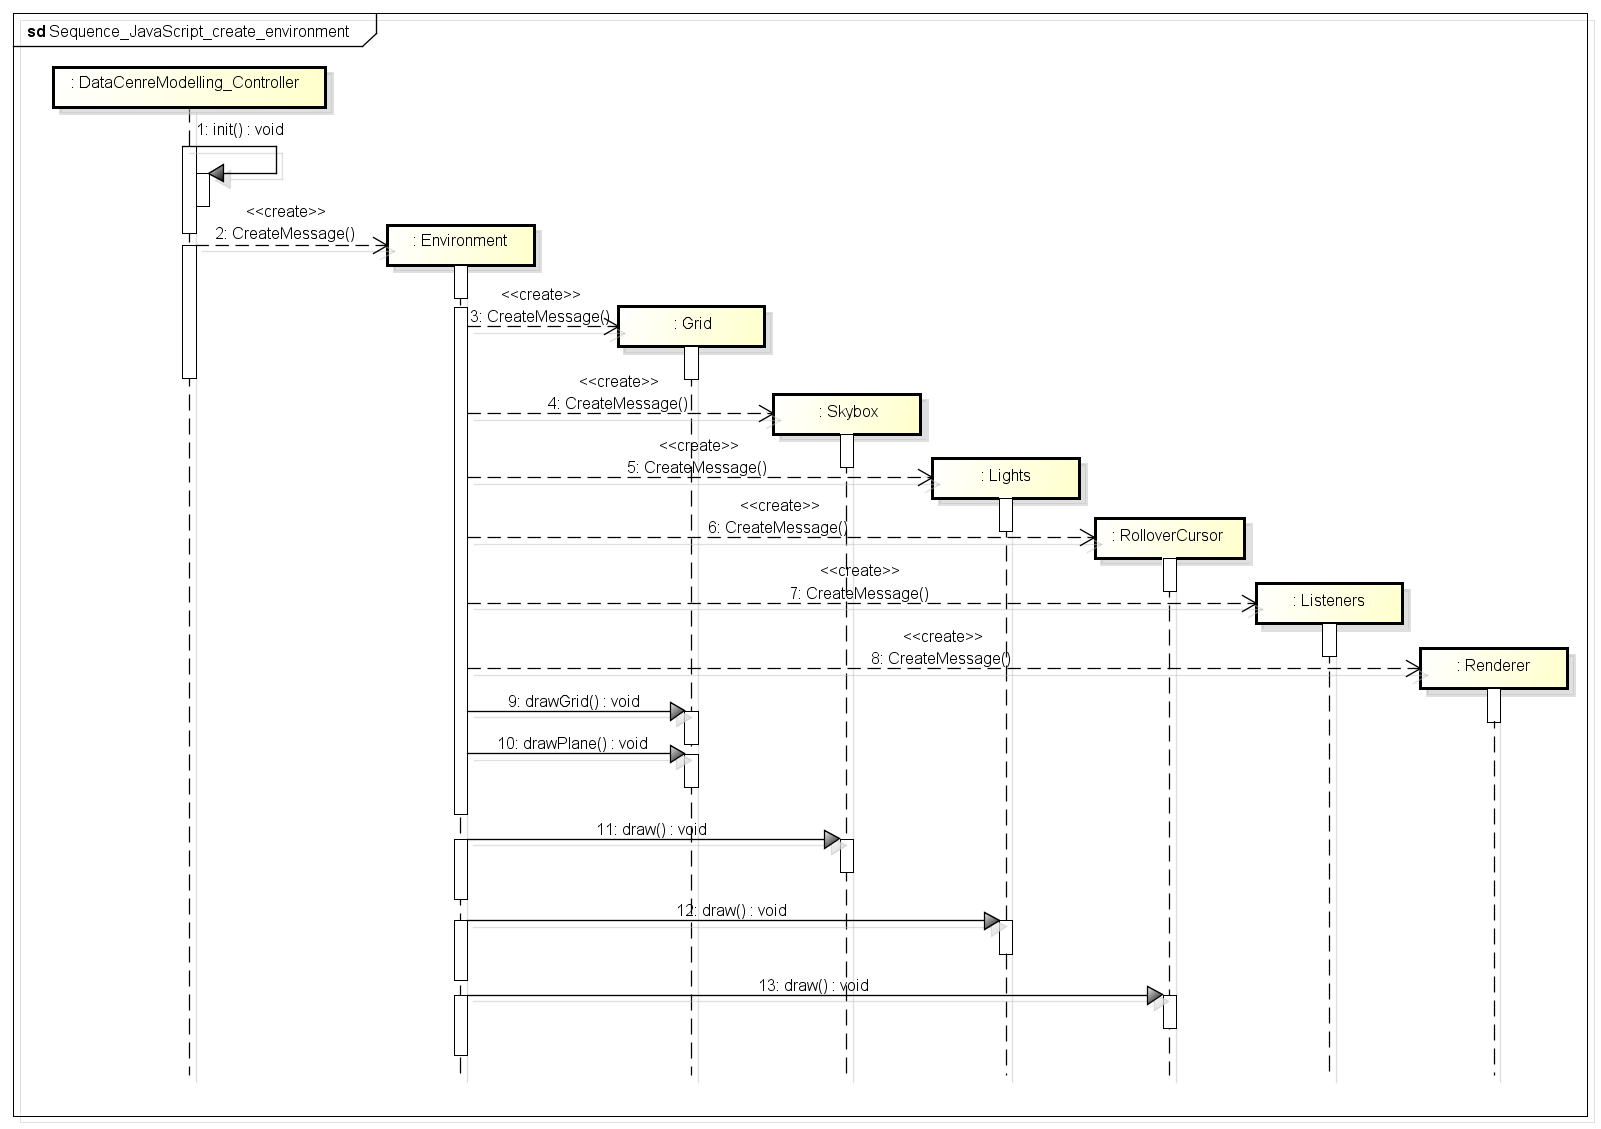
\includegraphics[width=5in]{Resources//Design_Diagrams//Sequence_JavaScript_create_environment.png}
\caption{UML Sequence diagram of the process of rendering the 3D visual environment on page load, showing interactions between JavaScript classes.}
\label{}
\end{figure}

\begin{figure}[H]
\centering
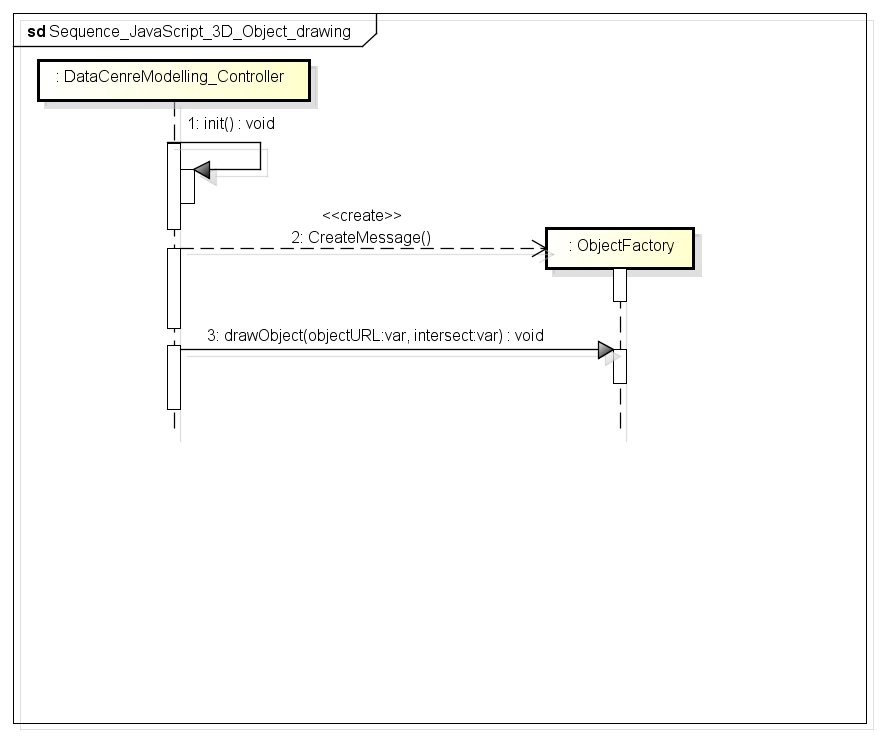
\includegraphics[width=5in]{Resources//Design_Diagrams//Sequence_JavaScript_3D_Object_drawing.png}
\caption{UML Sequence diagram of the process by which a 3D object is drawn by user interaction with the HTML view, concerning the involved JavaScript classes.}
\label{}
\end{figure}

\subsection{Back-end}

\begin{figure}[H]
\centering
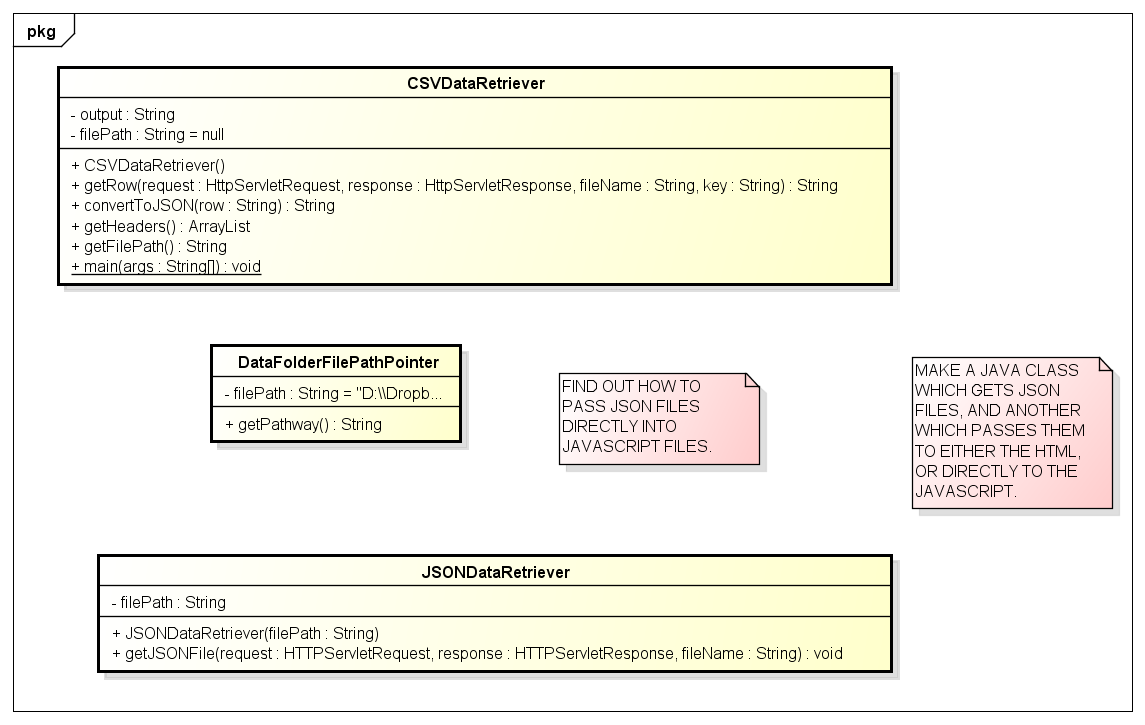
\includegraphics[width=5in]{Resources//Design_Diagrams//Class_Java Back-end.png}
\caption{}
\label{}
\end{figure}

\subsection{Support site}

\begin{figure}[H]
\centering
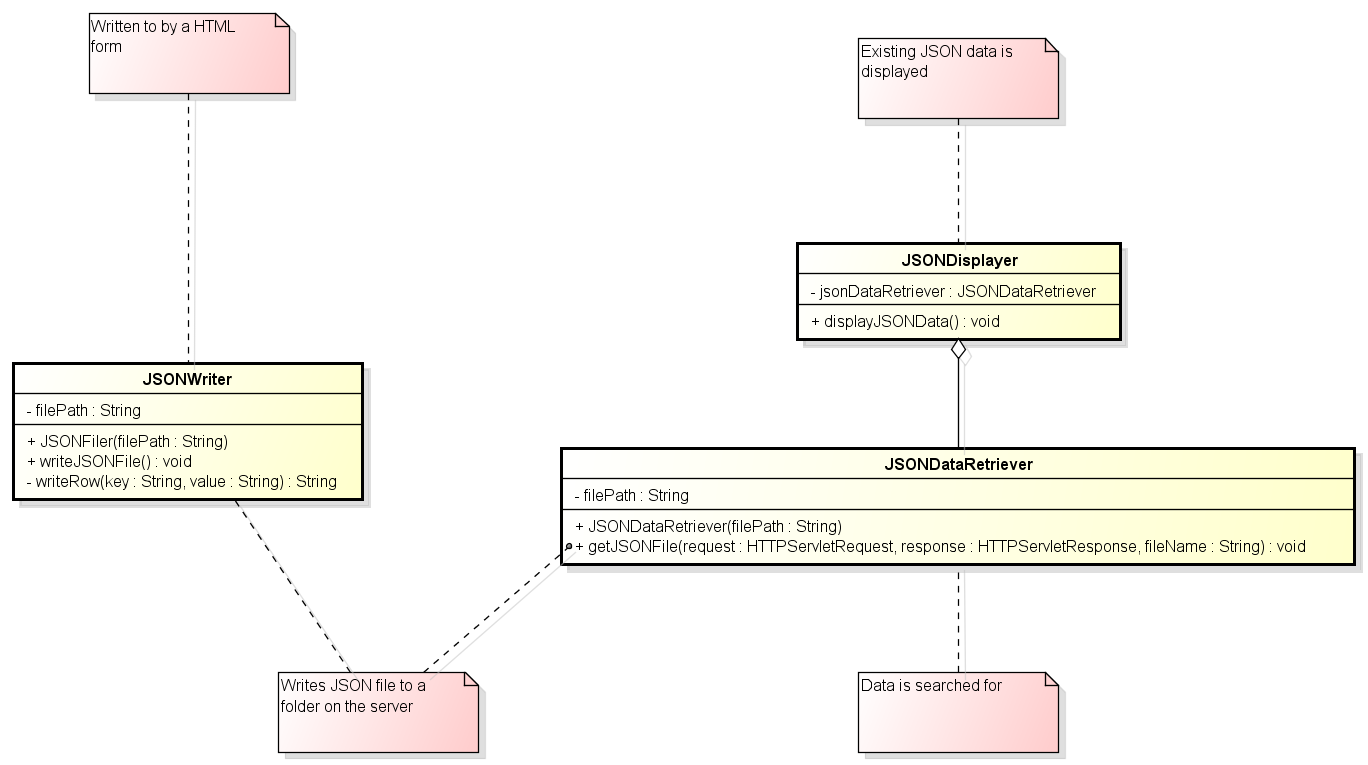
\includegraphics[width=5in]{Resources//Design_Diagrams//Class_Backend site java controller.png}
\caption{}
\label{}
\end{figure}

































%Everything else is depreciated
\iffalse

\section{Development of the Component-Database and the Logic-Engine Application Components}
\label{sec:DevelopmentOfTheComponentDatabaseAndTheLogicEngineApplicationComponents}


\subsection{Simplified Overview\textcolor{red}{[FROM PRESENTATION]}}
\label{sec:Methodology:SimplifiedOverview}
The application will be developed as a series of inter-operating sub-programs:

\begin{itemize}
\item The game interface.
    This consists of two components:
\begin{enumerate}
\item The programming interface: Ties all of the other sub-programs in the application together.

\item The Graphical User Interface, giving the user an intuitive, game like control and experience of the game
\end{enumerate}
\item The component database: containing information on anything the player can select and add to their data centre. 

\item The logic engine: A set of rules about the data centre, providing bonuses and penalties to the player based on their choices from the component database.
\end{itemize}

\begin{figure}[H]
\centering
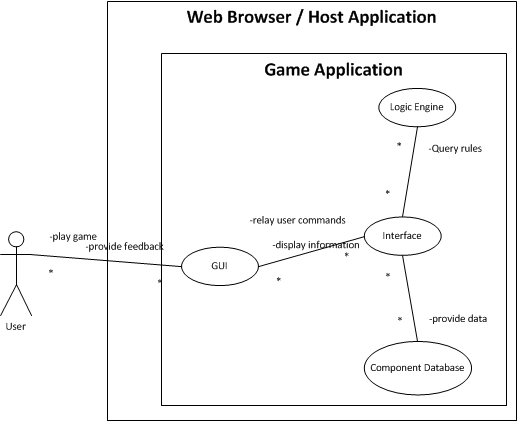
\includegraphics[width=5in]{Resources//Use Case Diagram.png}
\caption{A use-case diagram of the interactions between the sub programs.}
\label{fig:UseCaseDiagram}
\end{figure}

\subsection{Technical Overview\textcolor{red}{[FROM PRESENTATION]}}
\label{sec:Methodology:TechnicalOverview}
\subsubsection{The Component Database\textcolor{red}[FROM PRESENTATION]}
\label{sec:Methodology:TechnicalOverview:TheComponentDatabase}
This is a repository of all elements that can feasibly have an affect 
on the operation of the data centre. Examples include:

\begin{itemize}
\item Cooling systems
\item CPUs
\item Data traffic management algorithms
\item Operating times
\item Average ambient temperatures
\end{itemize}

For each of these, attributes are included, such as power
Consumption (which would be added to the overall power
consumption for the whole data-centre), purchasing cost, ideal operating 
temperature etc.

The Component Database is intended to be extensible, so that 
new technologies can be added As they become available.

Initially, an object oriented approach to the development of the database was taken
The justification of this approch is as follows:

\begin{itemize}

\item Generic classes can be used, which can be defined as being specific variations
 dependant on input parameters An example of this could be the considered to be the various
types of air conditioning system defined in section \ref{sec:ACriticalReviewOfReleventScientificAndEngineeringLiturature:StudiesIntoTheEnvironmentalEffectsAndEnergyEffiencyOfDataCenters:TheDifferentTypesOfAirConditioningEquipmentForITEnvironments}
\cite{TonyEvansTheDifferentTypesOfAirConditioningEquipmentForITEnvironmentsWhitePaper};

\item A switch-case construct could be used to define parameters supplied to an ``air conditioning system"
object at its construction, such as the devices spacial footprint, location within the room and a number 
used to define whether it is an air cooled system, a glycol cooled system, or another.

\end{itemize}

\subsubsection{Isolated testing of the Component Database}

\subsubsection{The Logic Engine\textcolor{red}{[FROM PRESENTATION]}}
\label{sec:Methodology:TechnicalOverview:TheLogicEngine}
It Will be written as a knowledge base, prototyped in a logical programming language such as Prolog or Simulink, before being written in a way that it can be used by the program interface.

Queries will consist of an entity in the Component Database being checked against the list of predicates in the Logic Engine's knowledge base. 

For example, if the user chooses a component, $A$, that has a maximum operating temperature, $T_{max}$, and then the user tries to add another component, $B$ which will raise the ambient temperature, $T_{amb}$ of the data centre above $T{max}$ , then the logic engine will prevent the Program Interface from allowing the user to add $B$.

%\begin{equation}
%\begin{split}
%&P_1 \models A \Rightarrow T_{max} \\
%&P_2 \models B \Rightarrow T_{amb} > T_{max} \\
%&C \models A \and \neg B \Rightarrow T_{amb} < %T_{max} \\
%\end{split}
%\end{equation}

\begin{equation}
\begin{split}
&P_1 \equiv A \Rightarrow T_{max} \\
&P_2 \equiv B \Rightarrow T_{amb} > T_{max} \\
&C \equiv A \land \neg B \Rightarrow T_{amb} < T_{max}
\end{split}
\end{equation}


The testing phase of this element will consist of querying a series of predicates in the knowledge base against dummy data. Once the Logic Engine works to a satisfactory extent, it will be integrated into the Testing Interface and tested against data in the Component Database.

The Logic Engine is intended to be extensible, so that if new principles are discovered that apply, they can be included.

\subsubsection{Isolated testing of the Logic Engine}

\subsubsection{The Program Interface\textcolor{red}{[FROM PRESENTATION]}}
\label{sec:Methodology:TechnicalOverview:TheProgramInterface}
This serves as the interface allowing the user to communicate with 
the program via the GUI, and for the program to query information on 
user selected components
against the logic engine.

It's development life-cycle will be in two stages:

\begin{enumerate}

\item The aforementioned “Testing Interface” will be developed in order to test the compatibility 
of the Component Database and the Logic Engine. As a test program, its input and output 
will primarily be through the command line.

\item The Testing interface will be further developed into the Program Interface by adding the
capacity for it to relay information between the other sub programs and the GUI.

\end{enumerate} 

The Program Interface will be written in JavaScript, allowing integration into a web page coded in HTML5 and CSS.

\subsubsection{Isolated testing of the Program Interface}

\subsubsection{The GUI\textcolor{red}{[FROM PRESENTATION]}}
\label{sec:Methodology:TechnicalOverview:TheGUI}
The GUI will be programmed to communicate with the program interface on the programming interface's terms. This allows multiple developments of the GUI, testing whether 2D or 3D GUIs work best with the game.

\begin{figure}[H]
\centering
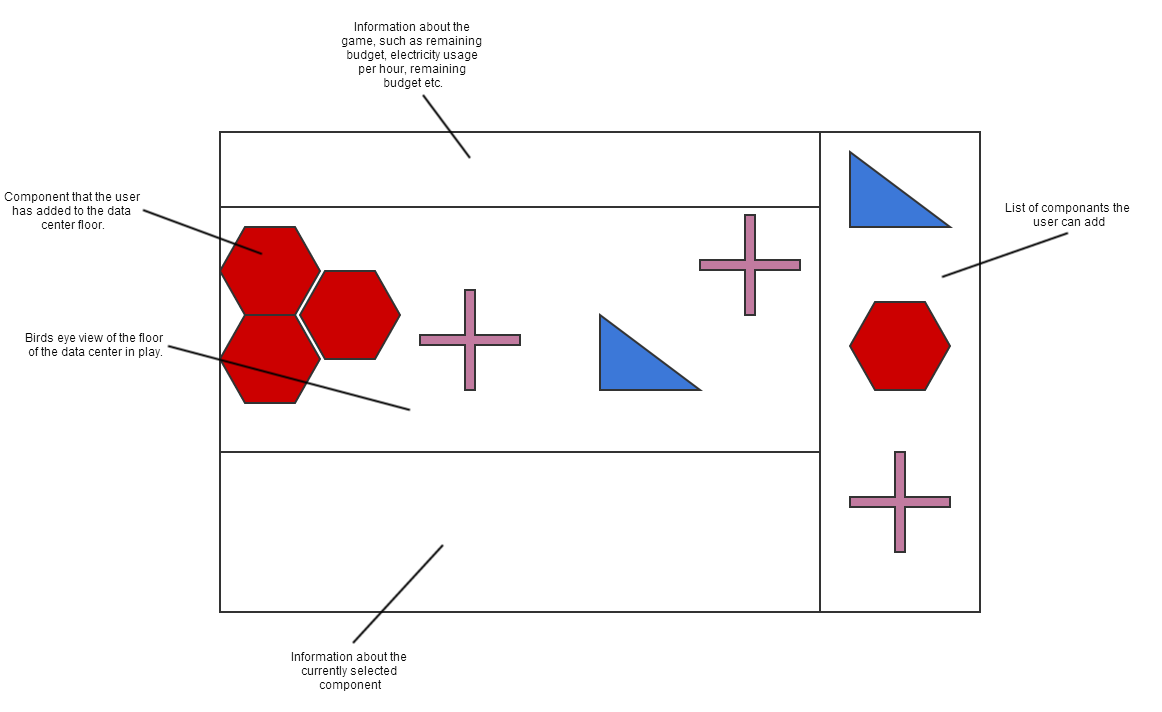
\includegraphics[width=7.25in]{Resources//GUI Mock up.png}
\caption{A mock up example of a potential GUI design, showing a top-down view of the \gls{data centre} floor, allowing users to place components from a list on the right hand side of the screen, with information about the component in the bottom pane, and general game information in the top pane.}
\label{fig:GUIMockUp}
\end{figure}

\subsubsection{Test Cycle One}
\label{sec:DevelopmentOfTheComponentDatabaseAndTheLogicEngineApplicationComponents:TestingOfTheComponentDatabaseAndTheLogicEngineViaTheTestInterface:TestCycleOne}

The first issue found was that...

This was corrected by performing the following actions:
\begin{itemize}
\item
\item
\item
\end{itemize}

The second issue found was that...

This was corrected by performing the following actions:
\begin{itemize}
\item
\item
\item
\end{itemize}

\section{Development of an Interface between the Component-Database and the Logic-Engine, and Development of a GUI}
\label{sec:DevelopmentOfAnInterfaceBetweenTheComponentDatabaseAndTheLogicEngineAndDevelopmentOfAGUI}

\subsection{Interface Development}
\label{sec:DevelopmentOfAnInterfaceBetweenTheComponentDatabaseAndTheLogicEngineAndDevelopmentOfAGUI:InterfaceDevelopment}
\textcolor{red}{The interface will be developed from the Test-Interface (section \ref{sec:DevelopmentOfTheComponentDatabaseAndTheLogicEngineApplicationComponents:TheTestInterface}). As such, this section may become obsolete and be removed.}

\subsection{The GUI}
\label{sec:DevelopmentOfAnInterfaceBetweenTheComponentDatabaseAndTheLogicEngineAndDevelopmentOfAGUI:TheGUI}
\textcolor{red}{Chronicling of the development of the GUI}

\subsection{Integration}
\label{sec:DevelopmentOfAnInterfaceBetweenTheComponentDatabaseAndTheLogicEngineAndDevelopmentOfAGUI:Integration}
\textcolor{red}{Integration of the all of the software components and the GUI together into a working program.}

\fi
% ------------------------------------------------------------------------
% -*-TeX-*- -*-Hard-*- Smart Wrapping
% ------------------------------------------------------------------------
\def\baselinestretch{1}

\chapter{Testing}
\label{chapter:Testing}

\def\baselinestretch{1.66}


%%% ----------------------------------------------------------------------

\textcolor{red}{[GIVE A CHAPTER DESCRIPTION]}

%%% ----------------------------------------------------------------------
\goodbreak

\section{Application Testing}
\label{sec:ApplicationTesting}

 \subsection{Test Cycle One}
 \label{sec:ApplicationTesting:TestCycleOne}
 
 \subsubsection{Tests}
 \label{sec:ApplicationTesting:TestCycleOne:Tests}
 \textcolor{red}{A series of tests, of different aspects, under different conditions.}
 \begin{enumerate}
 \item The following conditions were in place during this test:
 \begin{itemize}
 \item
 \item
 \item
 \end{itemize}
 
 The following issues were found to occur under these conditions:
 \begin{itemize}
 \item
 \item
 \item
 \end{itemize}
 \item The following conditions were in place during this test:
  \begin{itemize}
  \item
  \item
  \item
  \end{itemize}
  
  The following issues were found to occur under these conditions:
  \begin{itemize}
  \item
  \item
  \item
  \end{itemize}
 \end{enumerate}
 \subsubsection{Developments}
 \label{sec:ApplicationTesting:TestCycleOne:Developments}
 Owing to the findings of the tests performed in section \ref{sec:ApplicationTesting:TestCycleOne:Tests}, the following modifications were made to the application:
 \begin{enumerate}
 \item
 \item
 \item
 \end{enumerate}
 
 \subsection{Test Cycle Two}
 \label{sec:ApplicationTestinng:TestCycleTwo}
 
 \subsubsection{Tests}
 \label{sec:ApplicationTesting:TestCycleTwo:Tests}
 
 \subsubsection{Developments}
 \label{sec:ApplicationTesting:TestCycleTwo:Developments}
 
 \section{Integration of the application into the web-page for browser deployment\textcolor{red}{[FROM PRESENTATION SECTION 'Hosting']}}
 \label{sec:Methodology:TechnicalOverview:Hosting}
 The game will be hosted on a web server page to allow as many
 users as possible to access it.
 
 Furthermore, the game may later be developed into a mobile app by wrapping it using software such as PhoneGap \cite{PhoneGap}, allowing for the greatest possible cross-platform access to it. 
% ------------------------------------------------------------------------
% -*-TeX-*- -*-Hard-*- Smart Wrapping
% ------------------------------------------------------------------------
\def\baselinestretch{1}

\chapter{Project Evaluation and Discussion}
\label{chapter:Evaluation}

\def\baselinestretch{1.66}


%%% ----------------------------------------------------------------------

\textcolor{red}{[GIVE A CHAPTER DESCRIPTION]}

%%% ----------------------------------------------------------------------
\goodbreak

 \section{Critical Analysis of the Application}
 \label{sec:CriticalAnalysisOfTheApplication}

% ------------------------------------------------------------------------

\clearpage
\printglossaries

\clearpage
%\setlinespacing{1.44}
%\bibliographystyle{amsplain}
\bibliographystyle{apalike}
\bibliography{DissoReferences}

%#### Include any appendix below #####
\appendix
\include{AppendixA}
%\include{AppendixB}



% =================================================================


\end{document}
% ------------------------------------------------------------------------
